\documentclass[11pt]{article}

\usepackage[a4paper,margin=1in]{geometry}
\usepackage[T1]{fontenc}
\usepackage[utf8]{inputenc}
\usepackage{lmodern}
\usepackage{textcomp}
\usepackage{graphicx}
\usepackage{booktabs}
\usepackage{longtable}
\usepackage{tabularx}
\usepackage{pdflscape}
\usepackage{fancyvrb}
\usepackage{enumitem}
\usepackage{hyperref}
\usepackage{xcolor}
\usepackage[numbers,sort&compress]{natbib}

\hypersetup{
  colorlinks=true,
  linkcolor=blue!55!black,
  citecolor=blue!55!black,
  urlcolor=blue!55!black
}

\graphicspath{{../figures/generated/}{../figures/}}

\newcommand{\modelcount}{19}
\DefineVerbatimEnvironment{pseudocode}{Verbatim}{
  fontsize=\scriptsize,
  frame=single,
  framesep=6pt,
  rulecolor=\color{black!25}
}

\title{Satellite Embedding: A Review}
\author{Draft Survey Workspace}
\date{\today}

\begin{document}

\maketitle

\begin{abstract}
Satellite embeddings have become a practical interface between large-scale Earth observation data and downstream geospatial analysis, yet the literature is still organized mainly around foundation models rather than the embeddings they produce. This review reframes the area from an embedding-centered perspective. We first define satellite embeddings as reusable latent representations derived from satellite or multimodal Earth observation data, and organize existing methods along three axes: model family, data and modality support, and deployment mode. We then consolidate \modelcount{} representative models into a unified dossier covering publication source, authorship, spatial scale, temporal semantics, architecture, pretraining signal, embedding dimensionality, runtime behavior, and code or artifact availability. Next, we outline an application-oriented benchmark agenda spanning classification, segmentation, regression, and retrieval, with a small-area comparative protocol that can be executed across both on-the-fly encoders and precomputed embedding products. Finally, we describe an interactive system layer that exposes these models through a lightweight explorer for region selection, model comparison, and rapid downstream experimentation. The resulting review is intended to serve simultaneously as a technical reference, an empirical evaluation framework, and a reproducible software entry point for the satellite embedding community.

\end{abstract}

\section{Introduction}

Earth observation is entering a representation-first stage. Open satellite constellations, long-running public archives, and large pretraining corpora have accelerated the development of remote sensing foundation models, while recent surveys have documented a rapid shift from vision-only pretraining pipelines toward multimodal, generalist, and task-adaptive Earth observation systems \citep{survey1,survey3,survey4}. By 2025, models such as SkySense++ were already reporting consistent gains across classification, detection, and segmentation on 12 Earth observation tasks in 7 domains, illustrating how quickly the field is moving from narrow benchmark models toward reusable geospatial representations \citep{skysensepp}. At the same time, new productized representations such as GSE and TESSERA suggest that the field is no longer defined only by trainable checkpoints; it is increasingly also defined by reusable embedding layers that can be queried, indexed, and redistributed as geospatial products \citep{gse,tessera}.

This recent surge did not emerge in isolation. Satellite embeddings inherit a longer remote sensing representation-learning trajectory that begins well before the current foundation-model vocabulary. Earlier Earth observation pipelines were dominated by hand-crafted spectral indices, texture descriptors, bag-of-visual-words features, and shallow classifiers designed for scene classification, land-cover mapping, or target detection. The first major break came when convolutional neural networks were transferred from natural images into remote sensing, making it possible to learn hierarchical spatial features directly from high-resolution imagery rather than engineering them manually. Early CNN-based scene classification work showed that transfer learning could outperform traditional remote sensing descriptors and established a practical template for representation reuse in Earth observation \citep{castelluccio2015}. In retrospect, those CNN feature extractors were the immediate ancestors of today's satellite embeddings: users often discarded the final classifier and reused intermediate or pooled activations as generic scene descriptors.

The second break was infrastructural as much as architectural. Free and open satellite archives, especially Landsat and Sentinel, dramatically increased the scale of accessible Earth observation data; platforms such as Google Earth Engine reduced the friction of assembling geographically distributed training corpora; and commodity GPU clusters made it feasible to train larger encoders on longer temporal stacks \citep{gee2017}. These conditions changed the field from one centered on carefully curated benchmark datasets to one capable of pretraining on global or continental imagery streams. Self-supervised learning then provided the methodological bridge. Seasonal Contrast demonstrated that remote sensing models could be pretrained directly from uncurated satellite time series without dense manual annotation, while the broader success of vision transformers shifted the community toward token-based architectures that scale more naturally with patch representations, masking, and multimodal fusion \citep{seco2021,vit2021,vitrs2021}. Once these ingredients were in place, the transition from task-specific CNN encoders to reusable Earth observation representation models became much faster.

The third break was the consolidation of those ingredients into model families that look recognizably ``foundation-like'' from a remote sensing perspective. Transformer backbones enabled patch masking and reconstruction objectives, as seen in SatMAE and ScaleMAE; contrastive learning made semantic alignment and retrieval practical, as seen in RemoteCLIP; and modality-aware tokenization opened the door to sensor-flexible encoders such as Prithvi, DOFA, Galileo, and later multimodal systems \citep{satmae,scalemae,remoteclip,prithvi,dofa,galileo}. At the same time, product-serving workflows matured: instead of exposing only a checkpoint, some systems began serving annual or static embedding layers that could be sampled directly in mapping pipelines. That shift matters because it changes the unit of use. The operational object is no longer only a model to fine-tune, but also a representation product to query, compare, and fuse with labels or side information.

This evolution is important because remote sensing is not merely another image domain. Earth observation representations must absorb multi-resolution and multi-sensor inputs, spectral bands beyond RGB, repeated observations through time, strong geographic and seasonal dependence, and large shifts in coverage, cloud conditions, and annotation density. As emphasized by recent surveys, the gap between natural-image assumptions and remote sensing practice remains substantial, especially when models are transferred across sensors, regions, and tasks \citep{survey1,survey3,survey4}. A recent NASA primer makes the same point from a deployment perspective: benchmark scores alone are insufficient for model selection in Earth observation, because practitioners must also reason about pretraining data, tokenization, architectural choices, and downstream use-case fit \citep{primer_eo}. In other words, the central question is no longer only whether a remote sensing foundation model exists, but what kind of representation it exposes, under what sensing assumptions, and with what practical trade-offs.

That framing motivates the core viewpoint of this review. In operational use, practitioners rarely begin with a full training recipe or a backbone diagram. They begin with an \emph{embedding}: a pooled scene vector for classification or retrieval, a dense token grid for segmentation, an annual embedding field for wide-area mapping, or a shared latent space aligned with text and metadata. The same backbone can induce very different reusable objects depending on pooling rules, temporal summarization, modality routing, adapter design, or product distillation. Conversely, models trained with different pretraining objectives can occupy a similar practical niche if both yield compact, transferable representations. This is why contrastive image-text systems such as RemoteCLIP \citep{remoteclip}, masked autoencoder lineages such as SatMAE and SatMAE++ \citep{satmae,satmaepp}, multimodal generalists such as Prithvi and DOFA \citep{prithvi,dofa}, and precomputed global embedding products such as GSE and TESSERA \citep{gse,tessera} should be read not as isolated threads, but as members of a common satellite embedding ecosystem.

An embedding-centered review is also useful because it makes evaluation more realistic. What matters for downstream use is not only whether a model reaches a high score on one benchmark, but whether its representation is robust, spatially appropriate, temporally interpretable, and easy to deploy in real mapping workflows. These issues are becoming more visible as the field matures. REOBench, for example, reports that current Earth observation foundation models can experience substantial degradation under realistic corruptions, with performance drops ranging from less than 1\% to more than 20\% depending on the task, architecture, and perturbation type \citep{reobench}. Such evidence reinforces the need for a review that does more than list models. It must connect model families to sensing regimes, output forms, robustness expectations, and application scenarios.

This review therefore adopts an explicitly embedding-centered scope. We focus on reusable latent representations derived from satellite and closely related Earth observation data, rather than on remote sensing foundation models in the abstract. Our aim is to bridge three levels that are often separated in the literature: the model paper, the benchmark protocol, and the deployment-facing software artifact. Concretely, the survey makes four contributions:

\begin{enumerate}[leftmargin=1.6em,label=(\roman*)]
  \item it defines a review-specific concept of \emph{satellite embedding} and proposes a unified taxonomy spanning model family, sensing modality, temporal semantics, output granularity, and deployment form;
  \item it assembles a structured dossier for the \modelcount{} canonical models currently exposed in the \texttt{rs-embed} workspace, including publication metadata, supported sensors, spatial resolution, architecture, output dimensionality, and practical deployment characteristics;
  \item it links the model landscape to application-facing use by organizing downstream tasks, outlining a consistent small-area evaluation protocol, and clarifying where different embedding families are likely to be strong or fragile;
  \item it turns the review into a living research artifact by pairing the literature synthesis with generated figures, benchmark scaffolding, and a lightweight interactive explorer for rapid comparison and experimentation.
\end{enumerate}

The remainder of this paper follows that logic. Section~2 defines the concept and taxonomy of satellite embeddings. Section~3 reorganizes the model landscape into major families and provides a detailed catalog. Sections~4 and~5 move to applications and comparative evaluation. Section~6 introduces the interactive system layer, and Sections~7 and~8 discuss open questions and conclusions. The goal throughout is to make the review useful both as a scholarly synthesis and as a practical entry point for researchers who need to select, compare, and deploy satellite embedding models.

\section{Overall Landscape of Satellite Embeddings}

\subsection{Why an embedding-centered review?}

Most existing remote sensing foundation model surveys are organized around pretraining paradigms, modality combinations, or downstream tasks. That is useful for describing the broader field, but it is not the most natural entry point for practitioners. In operational use, the object that is actually reused is usually an embedding: a pooled scene vector, a dense token grid, an annual embedding field, or a joint multimodal latent space. This review therefore starts from the reusable representation layer rather than from the training recipe alone.

\subsection{What is a satellite embedding?}

In this review, a satellite embedding is a reusable latent representation derived from satellite or related Earth observation data and intended to support multiple downstream tasks beyond the pretraining objective. This definition intentionally includes both on-the-fly encoder outputs and precomputed embedding products. It excludes purely task-specific logits or handcrafted indices unless they are explicitly repackaged as a transferable representation layer.

Four representation forms appear repeatedly in the current literature:

\begin{enumerate}[leftmargin=1.4em]
  \item \textbf{Pooled scene vectors}, commonly exposed by transformer encoders for classification, regression, or similarity search.
  \item \textbf{Dense token grids}, which preserve local spatial structure and can support segmentation or dense retrieval.
  \item \textbf{Annual embedding fields}, where the representation is served as a spatial product rather than recomputed at inference time.
  \item \textbf{Joint multimodal spaces}, where the embedding aligns imagery with text, metadata, or additional sensor streams.
\end{enumerate}

\begin{figure}[t]
  \centering
  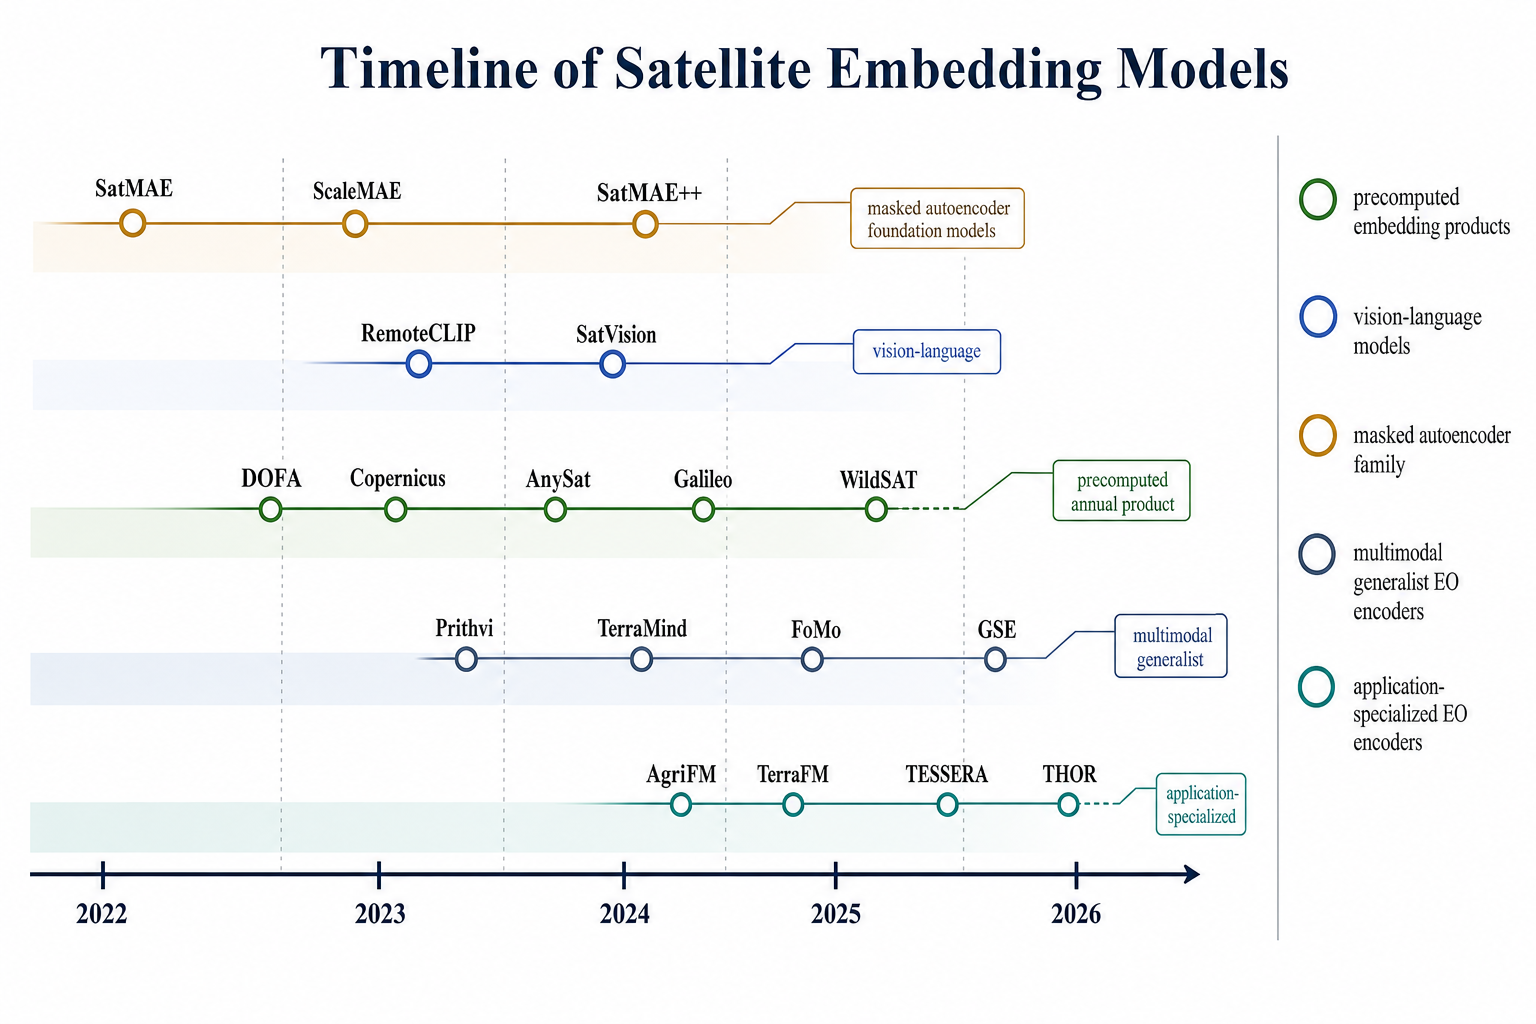
\includegraphics[width=\textwidth]{fig04_model_timeline_gptimage2_20260502.png}
  \caption{Model timeline view for the satellite embedding landscape. The figure emphasizes how precomputed products, masked autoencoder lineages, multimodal generalists, and application-specific encoders accumulate over time rather than appearing as a single homogeneous wave.}
  \label{fig:model-timeline}
\end{figure}

\subsection{Field evolution and major design axes}

For a remote sensing review, the overall story should appear before the detailed taxonomy. The field has evolved from early optical and masked-reconstruction pipelines toward broader multimodal, temporal, vision-language, and productized embedding systems. Figure~\ref{fig:model-timeline} provides this overall chronological view, which is easier for readers to absorb than a flat list of models.

We organize the literature along three orthogonal axes.

\paragraph{Model family.}
The first axis groups models by how the representation is learned and exposed: precomputed embedding products \citep{gse,tessera,copernicus}, vision-language systems \citep{remoteclip,wildsat}, masked autoencoder derivatives \citep{satmae,satmaepp,scalemae}, multimodal generalist encoders \citep{anysat,galileo,prithvi,terrafm,terramind,dofa}, and application-specialized Earth observation encoders \citep{agrifm,fomo,thor,satvision}.

\paragraph{Data and modality.}
The second axis captures the sensing substrate. Current models differ in optical-only versus optical-plus-SAR support, single-scene versus time-series modeling, fixed spectral assumptions versus wavelength-aware adaptation, and fine-resolution surface imagery versus coarse-resolution all-sky or atmosphere-linked sensing.

\paragraph{Deployment mode.}
The third axis separates systems that run a neural encoder at query time from systems that distribute the embedding directly as a product. This distinction is central for benchmarking because it changes runtime, storage, temporal flexibility, and failure modes. A precomputed product may offer extremely fast access but less temporal control, while an on-the-fly encoder may provide higher flexibility at the cost of data loading and GPU latency.

\begin{figure}[t]
  \centering
  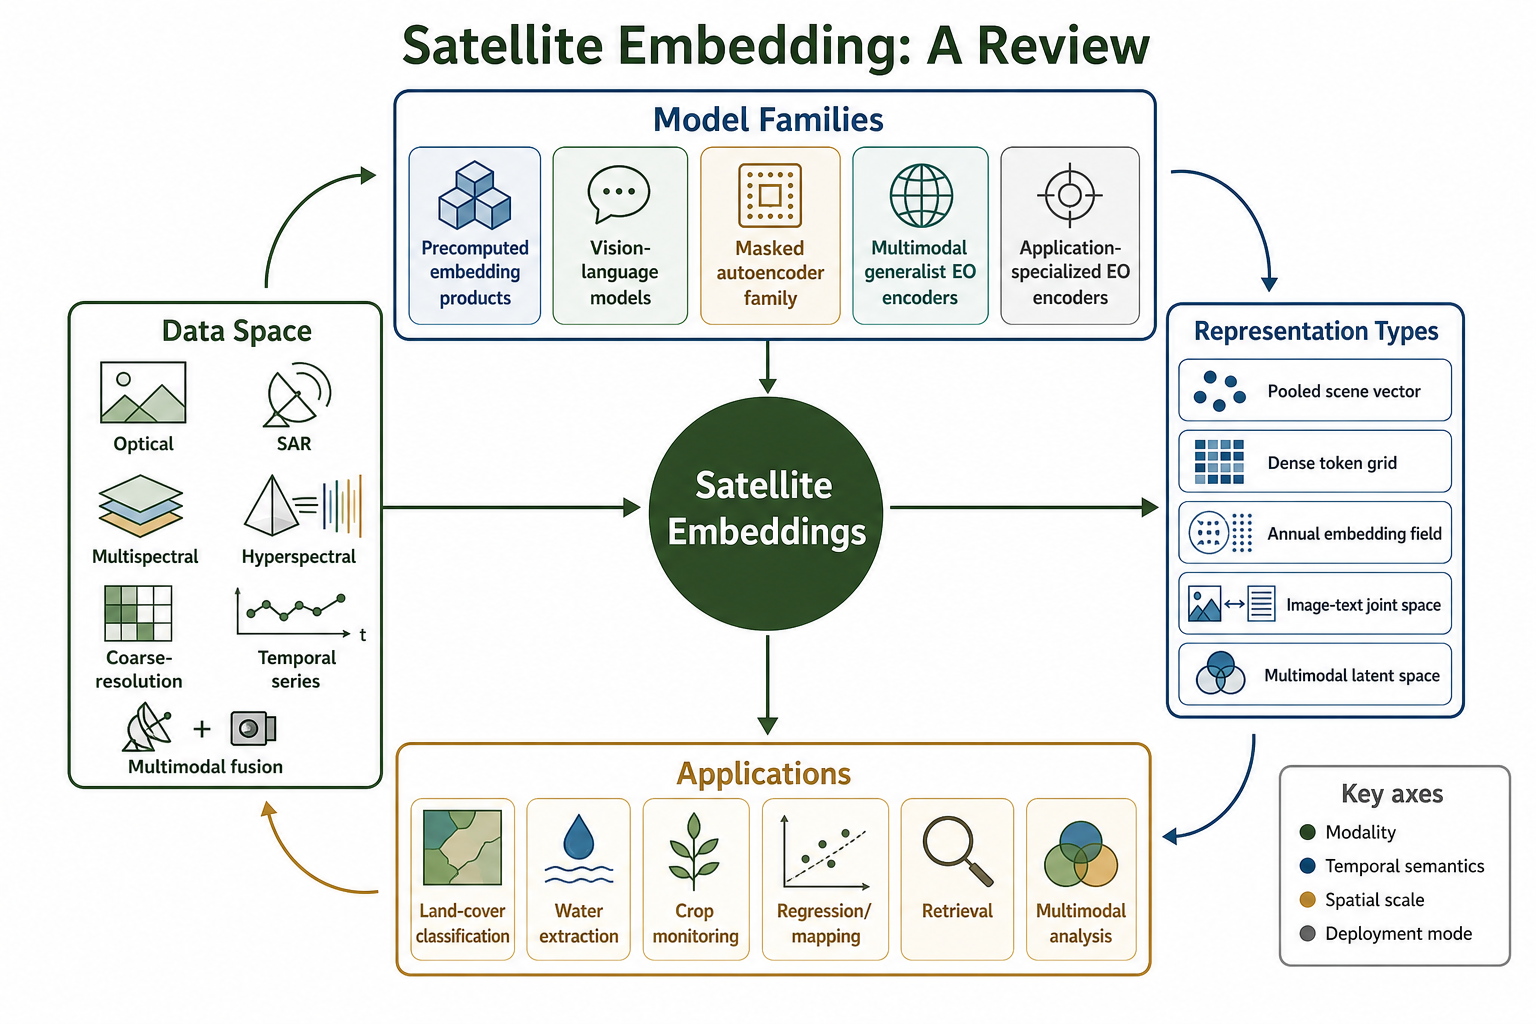
\includegraphics[width=\textwidth]{fig01_taxonomy_concept_map_gptimage2_20260502.png}
  \caption{Conceptual map of the satellite embedding landscape. The review is structured around four linked components: data space, model family, representation type, and downstream application. This framing is intentionally embedding-centered rather than checkpoint-centered.}
  \label{fig:taxonomy-concept-map}
\end{figure}

\subsection{Scope of this review}

An embedding-centered review should not simply relabel all remote sensing foundation models as satellite embeddings. Instead, the central question is whether the representation can serve as a general interface for downstream use. This criterion explains why annual products such as GSE and TESSERA belong in the same discussion as encoder checkpoints such as SatMAE++, AnySat, or TerraFM. All of them provide a transferable representation layer, but they differ sharply in spatial scale, temporal semantics, and deployment assumptions. Figure~\ref{fig:taxonomy-concept-map} summarizes this review logic in one diagram.

\section{Model Families of Satellite Embeddings}

The current \texttt{rs-embed} workspace exposes \modelcount{} canonical models, and the accompanying dossier records their publication metadata, supported sensors, output forms, and runtime summaries. For a review article, however, the reader should not face these as a flat inventory. A more natural structure is to first divide the field into a few broad model families, then summarize the common architecture and data logic of each family, and only after that return to a unified comparison table.

\subsection{Family I: Precomputed embedding products}

This family treats the embedding itself as a distributed geospatial product rather than as a checkpoint that must be run by the user. Examples include GSE, TESSERA, and Copernicus-style feature maps \citep{gse,tessera,copernicus}. Their main strengths are immediate access, large-area consistency, and low inference burden at use time. Their main limitations are temporal rigidity, storage requirements, and dependence on a fixed upstream production workflow.

\begin{figure}[t]
  \centering
  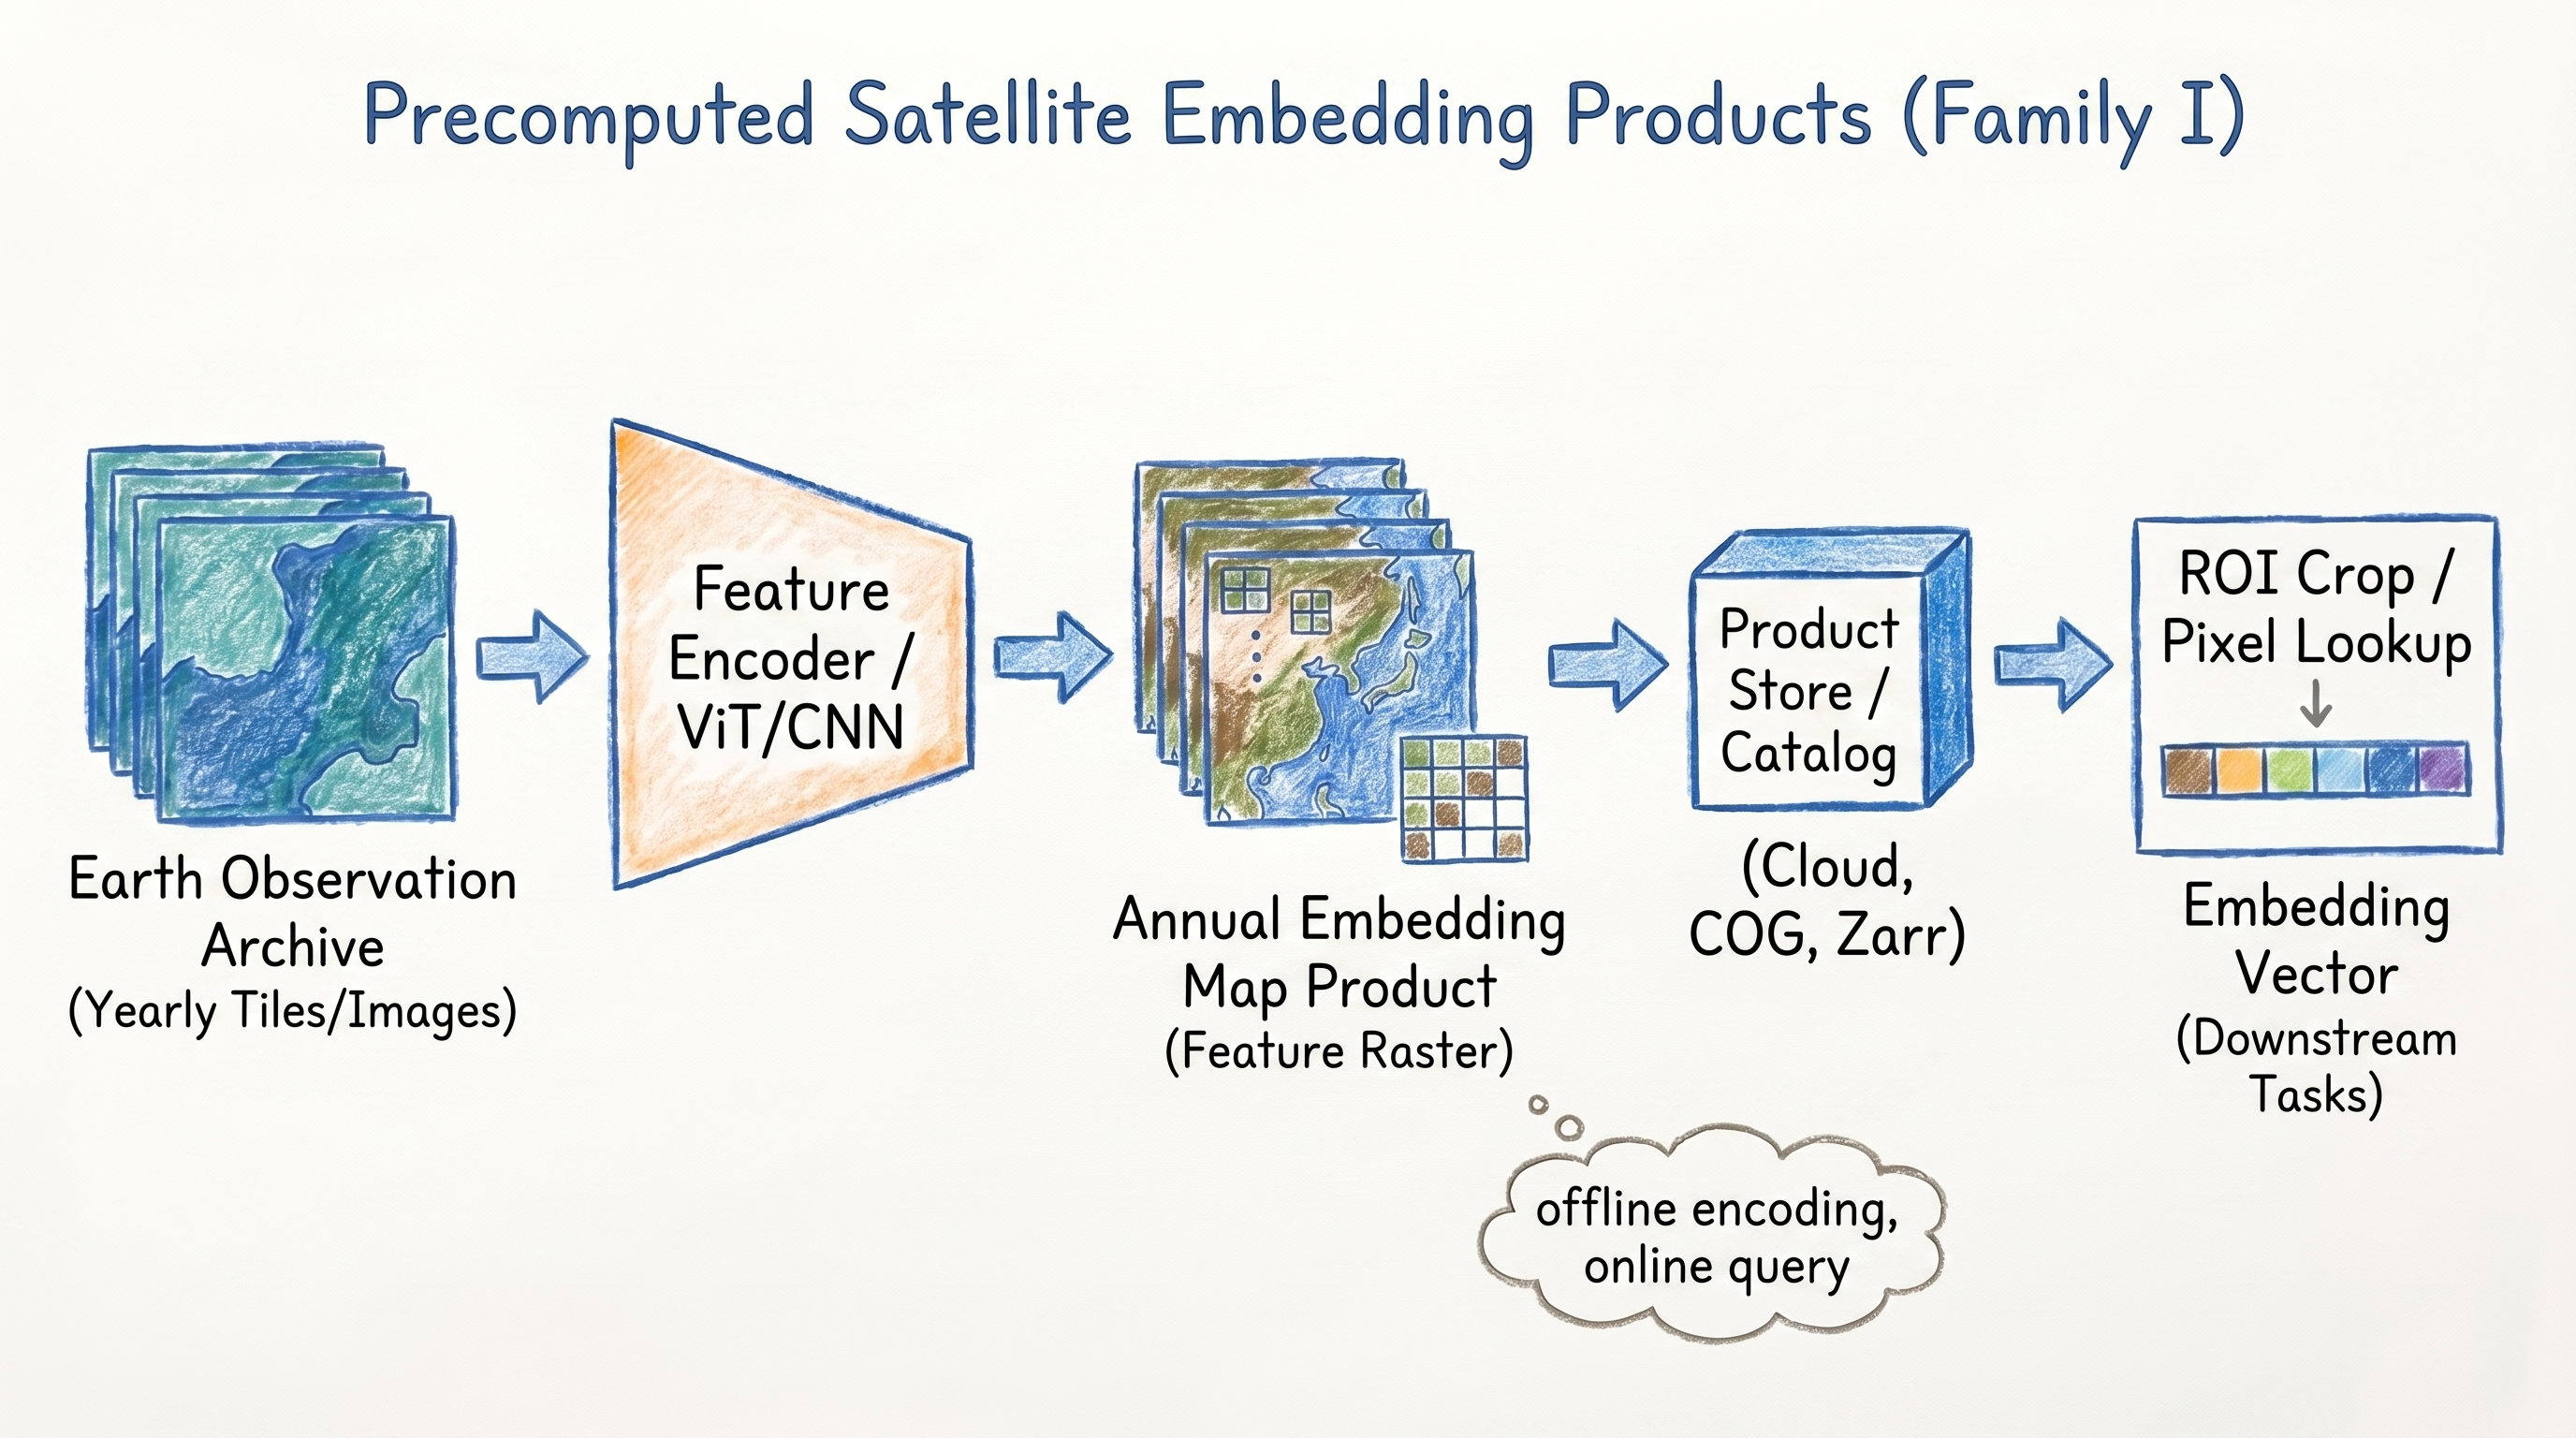
\includegraphics[width=\textwidth]{fig06_family_precomputed_products.png}
  \caption{Unified architecture sketch for precomputed embedding products. The dominant pattern is offline large-scale representation learning followed by annual or static embedding map generation, cataloging, and fast ROI-level feature access.}
  \label{fig:family-precomputed-products}
\end{figure}

\paragraph{Architecture summary.}
The central architectural move is to shift most computation from user-time to production-time. A large Earth observation archive is first condensed into a precomputed feature layer, often annualized or otherwise temporally summarized. Downstream users query that layer by ROI, tile, or pixel rather than rerunning the encoder. This architecture is especially attractive for wide-area monitoring and rapid transfer when access latency matters more than flexible temporal conditioning.

\paragraph{Pseudo-code template.}
\begin{pseudocode}
Input:
  Earth observation archive A
  temporal grouping rule T
  query ROI q

Offline stage:
  train encoder f_theta on large EO archive A
  for each period t in T:
      E_t <- f_theta(A_t)
      store embedding map E_t in product catalog

Online stage:
  crop or sample features z <- E_t[q]
  optionally pool or aggregate z
  train lightweight head g on sampled embeddings
  return prediction or retrieved features
\end{pseudocode}

\subsection{Family II: Masked autoencoder and pure vision encoders}

This group includes models such as SatMAE, SatMAE++, and ScaleMAE \citep{satmae,satmaepp,scalemae}. These methods are usually strongest when the goal is to learn transferable visual structure from optical or multispectral imagery through reconstruction-style pretraining. They are also among the clearest examples of the modern remote sensing foundation model trend, and many later systems can be interpreted as extending this lineage in scale, modality, or temporal handling.

\begin{figure}[t]
  \centering
  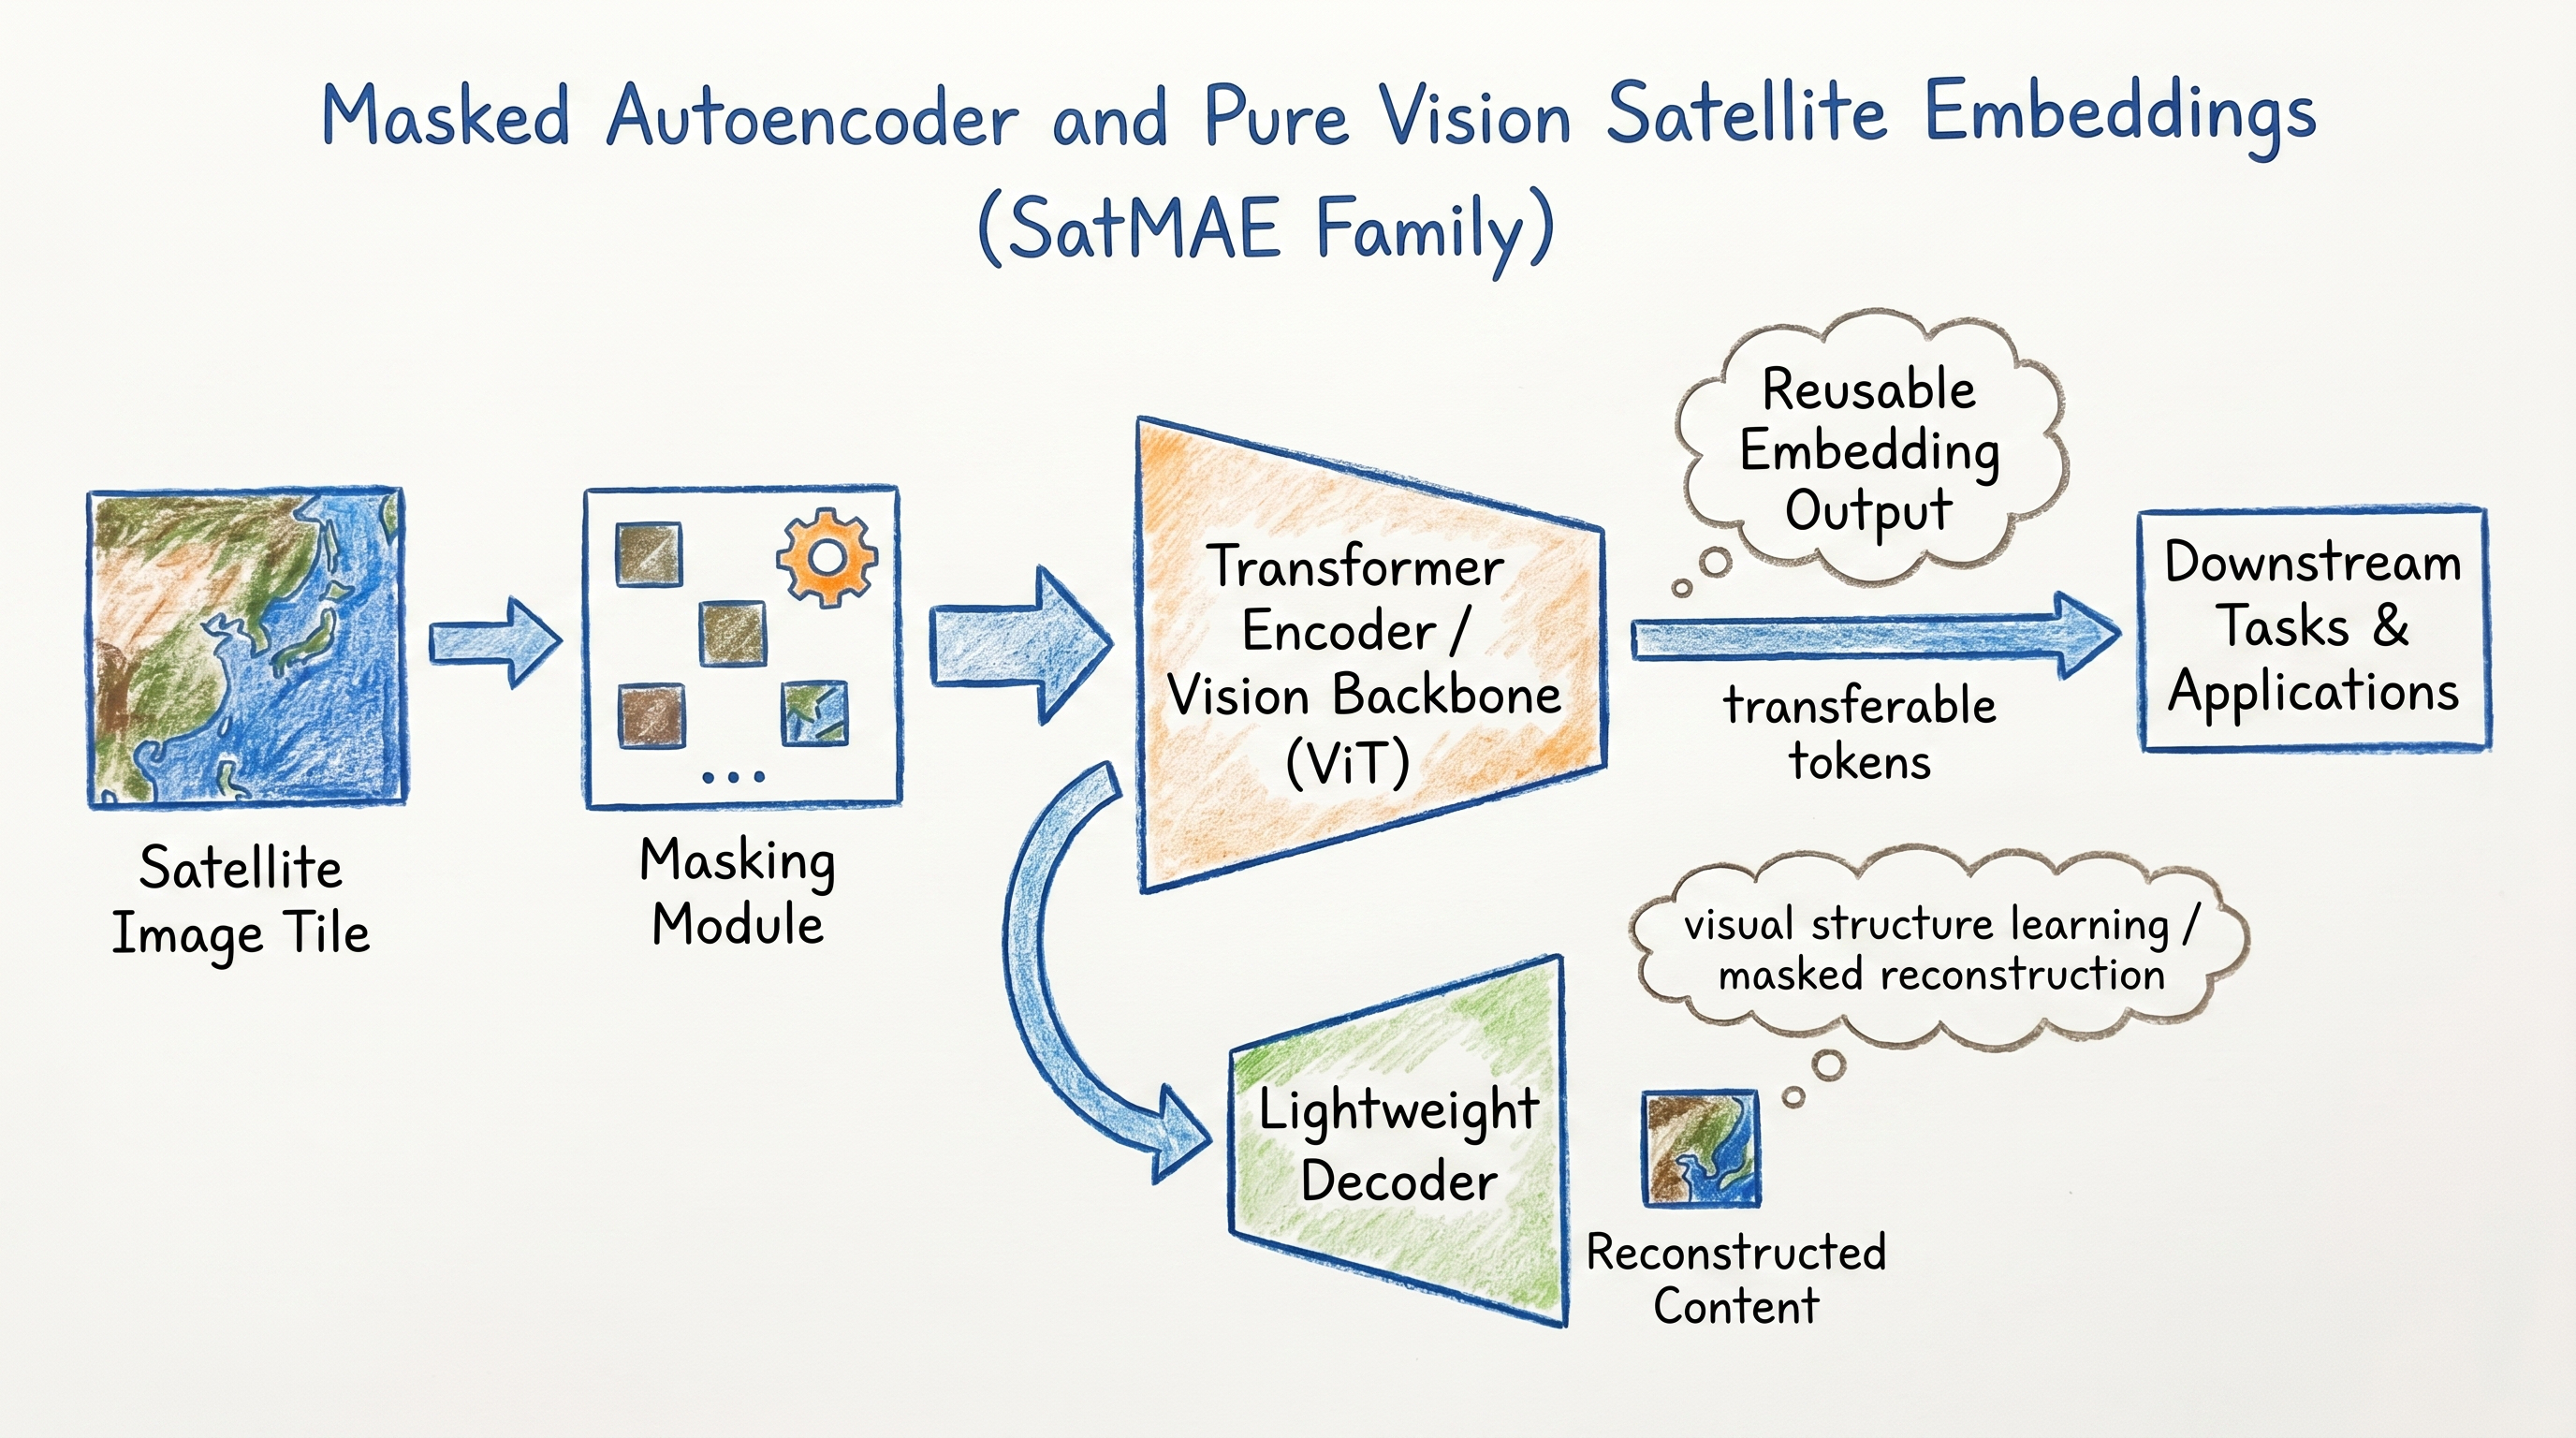
\includegraphics[width=\textwidth]{fig07_family_masked_autoencoder.png}
  \caption{Unified architecture sketch for masked autoencoder and pure vision satellite embedding models. Satellite tiles are partially masked, encoded by a transformer-style vision backbone, and supervised through reconstruction while the latent tokens are reused as transferable embeddings.}
  \label{fig:family-mae}
\end{figure}

\paragraph{Architecture summary.}
The shared logic is to learn a compact latent representation from partial visual evidence. Randomly masked patches, channels, or scale-aware inputs are passed through a vision encoder, while a reconstruction module encourages the latent space to preserve transferable visual structure. These embeddings often work well for classification and segmentation because they retain strong spatial cues without requiring language supervision.

\paragraph{Pseudo-code template.}
\begin{pseudocode}
Input:
  satellite tile x
  masking policy M

visible, hidden <- apply_mask(x, M)
tokens <- patch_embed(visible)
latent <- encoder(tokens)
recon <- decoder(latent, hidden)
loss <- reconstruction_loss(recon, x)
update model parameters

at inference:
  z_pool, z_grid <- read encoder representations
  return transferable embedding features
\end{pseudocode}

\subsection{Family III: Vision-language and cross-modal embeddings}

\begin{figure}[t]
  \centering
  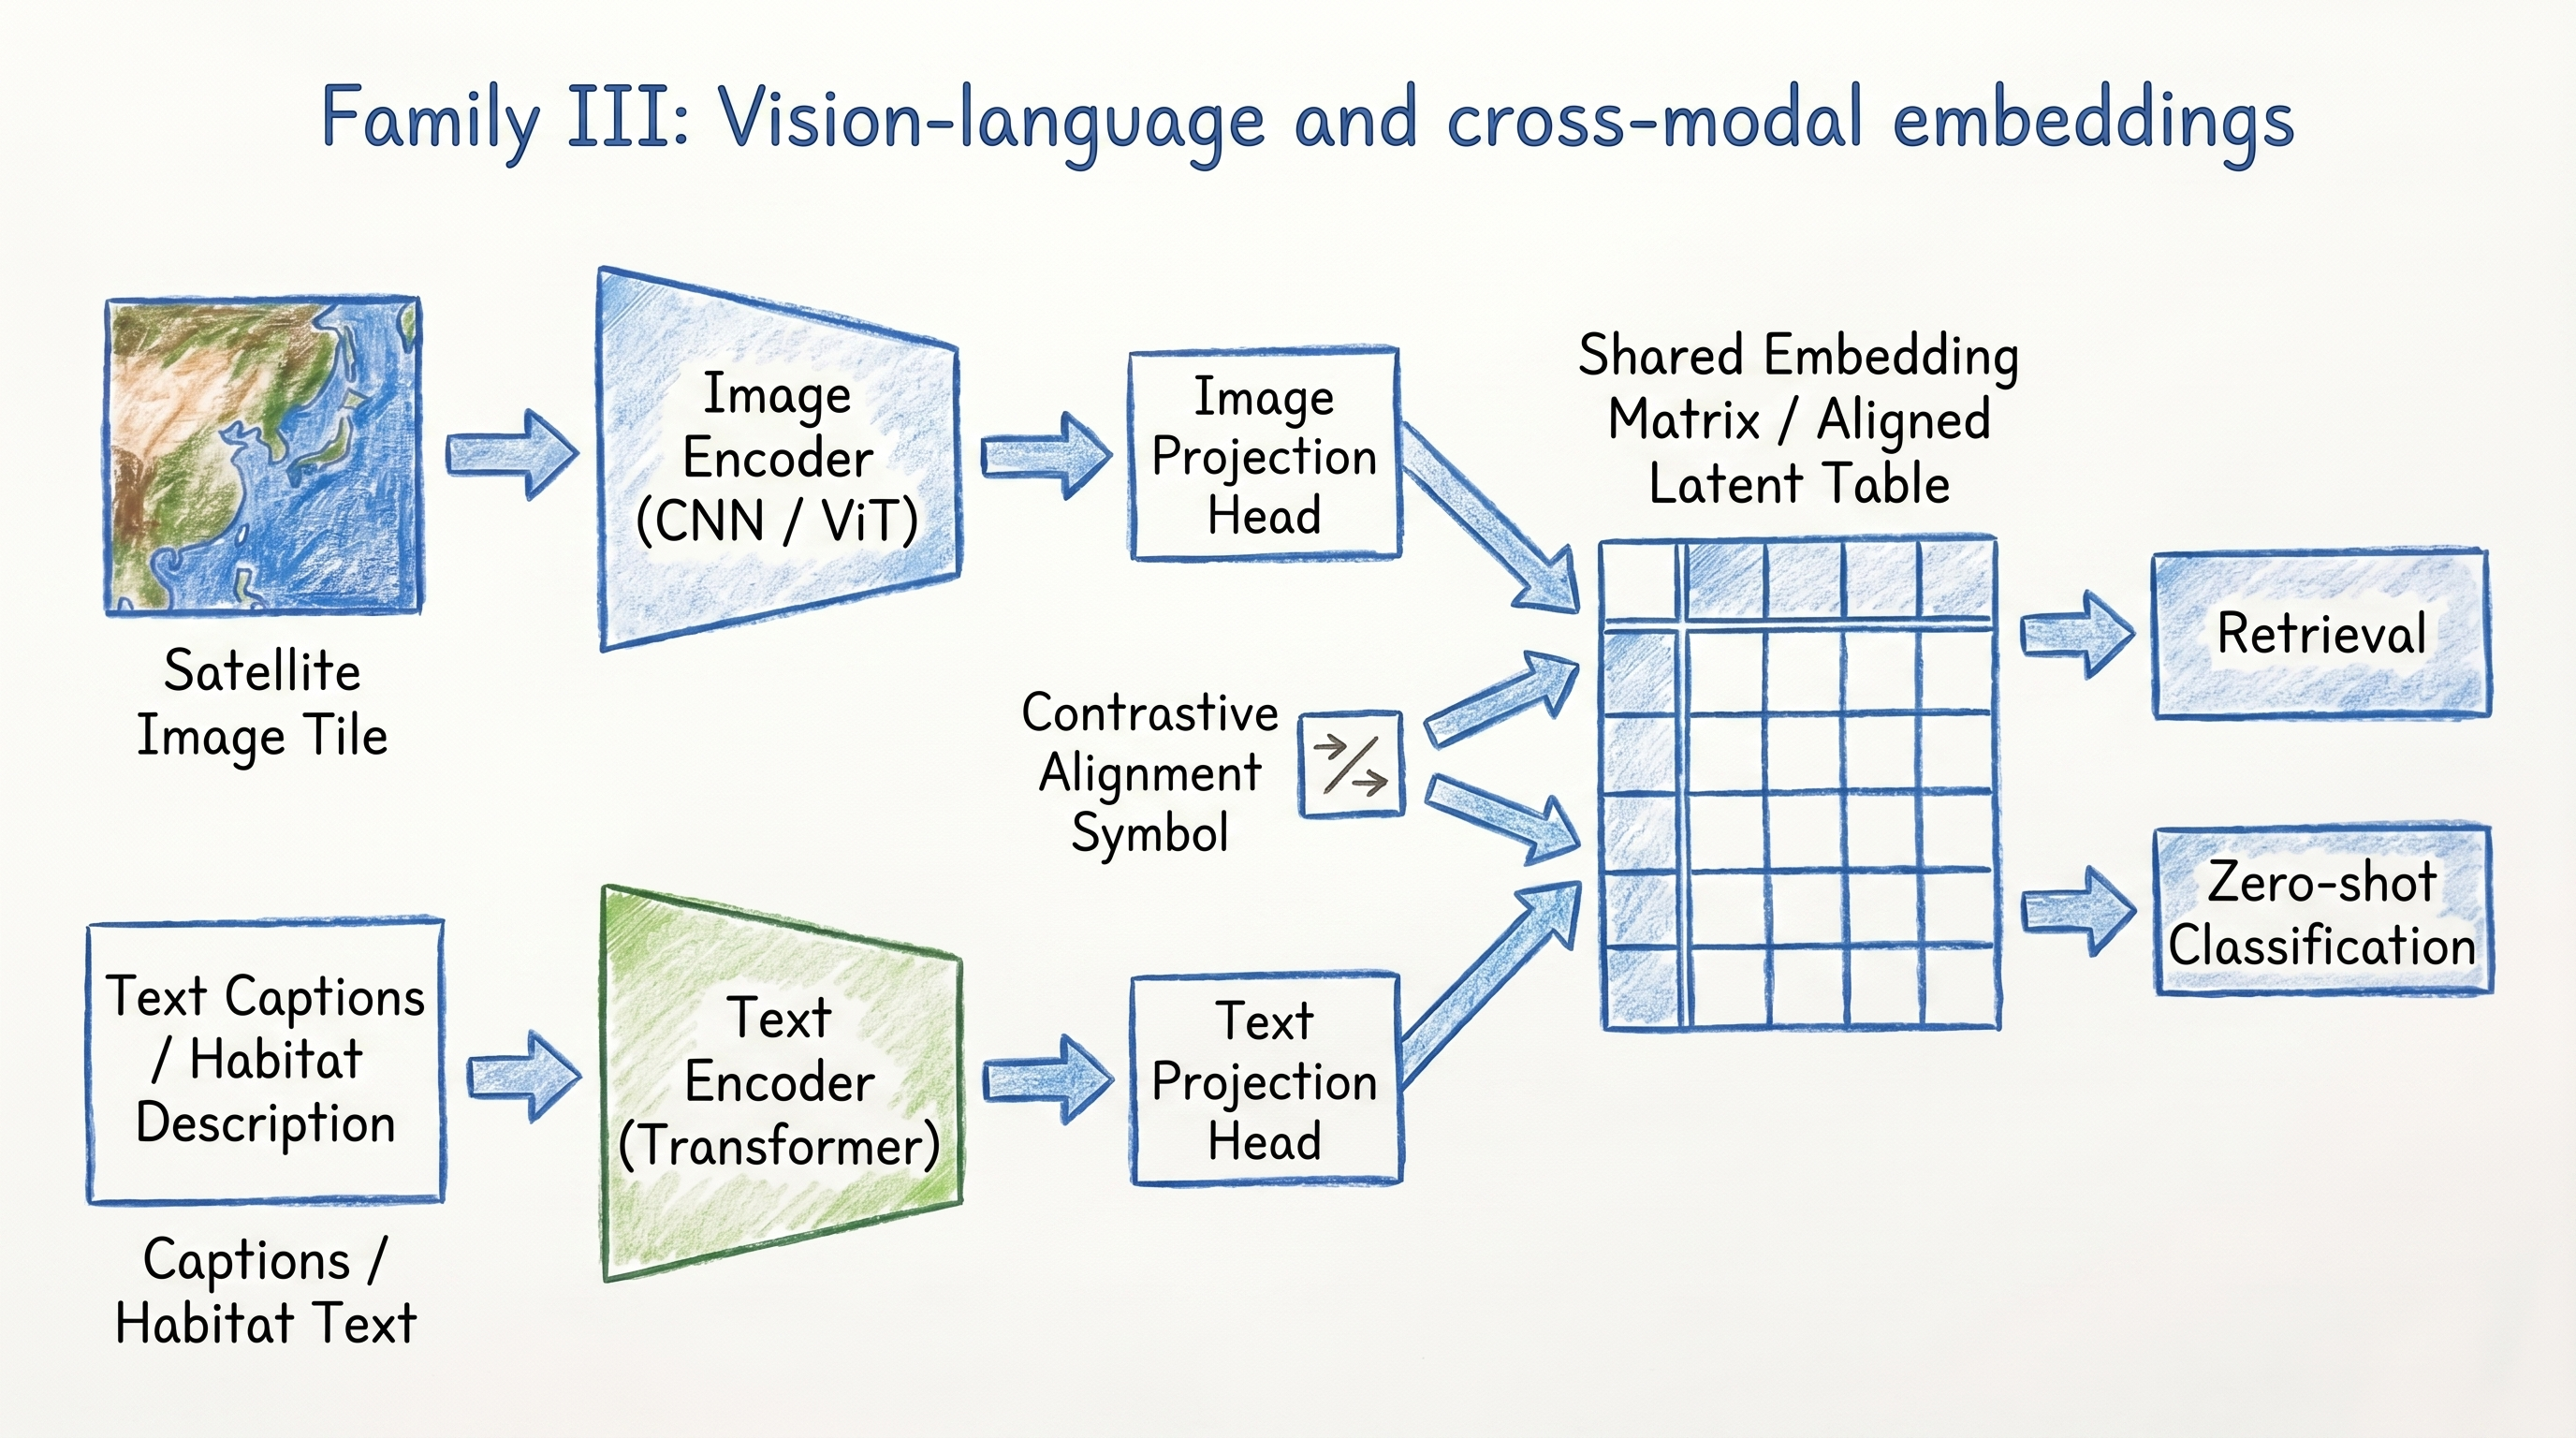
\includegraphics[width=\textwidth]{fig08_family_vision_language.png}
  \caption{Unified architecture sketch for vision-language and cross-modal satellite embeddings. The core pattern is image and text or ecological side-information encoding into a shared latent space trained by contrastive or alignment objectives.}
  \label{fig:family-vision-language}
\end{figure}

RemoteCLIP and WildSAT \citep{remoteclip,wildsat} illustrate the main idea of this family: satellite imagery is no longer embedded only against itself, but aligned with text, captions, habitat descriptions, or ecological side observations. This changes the representation from a purely visual latent space into a semantic one, which is why these models are especially important for retrieval, zero-shot transfer, and open-vocabulary interaction.

\paragraph{Architecture summary.}
Two encoders, one visual and one language or cross-modal, are trained to bring matched image-text or image-side-information pairs closer in a shared embedding space. The representation becomes useful not just for supervised transfer but also for semantic search and weakly supervised reasoning. In practice, this family adds a form of interpretability and open-vocabulary access that reconstruction-only models typically lack.

\paragraph{Pseudo-code template.}
\begin{pseudocode}
Input:
  satellite image x
  text or side-information y

z_img <- image_encoder(x)
z_txt <- text_encoder(y)
loss <- contrastive_alignment(z_img, z_txt)
update both encoders

at inference:
  use z_img for retrieval, zero-shot matching, or downstream probes
  optionally compare z_img against text prompt embeddings
\end{pseudocode}

\subsection{Family IV: Multimodal generalist EO encoders}

AnySat, Galileo, Prithvi, TerraFM, TerraMind, and DOFA represent a broader push toward modality-flexible or sensor-flexible Earth observation representation learning \citep{anysat,galileo,prithvi,terrafm,terramind,dofa}. These models are important because they move the field closer to a genuinely general EO representation space. Their distinguishing features include explicit handling of temporal stacks, wavelength metadata, modality routing, and cross-sensor alignment.

\begin{figure}[t]
  \centering
  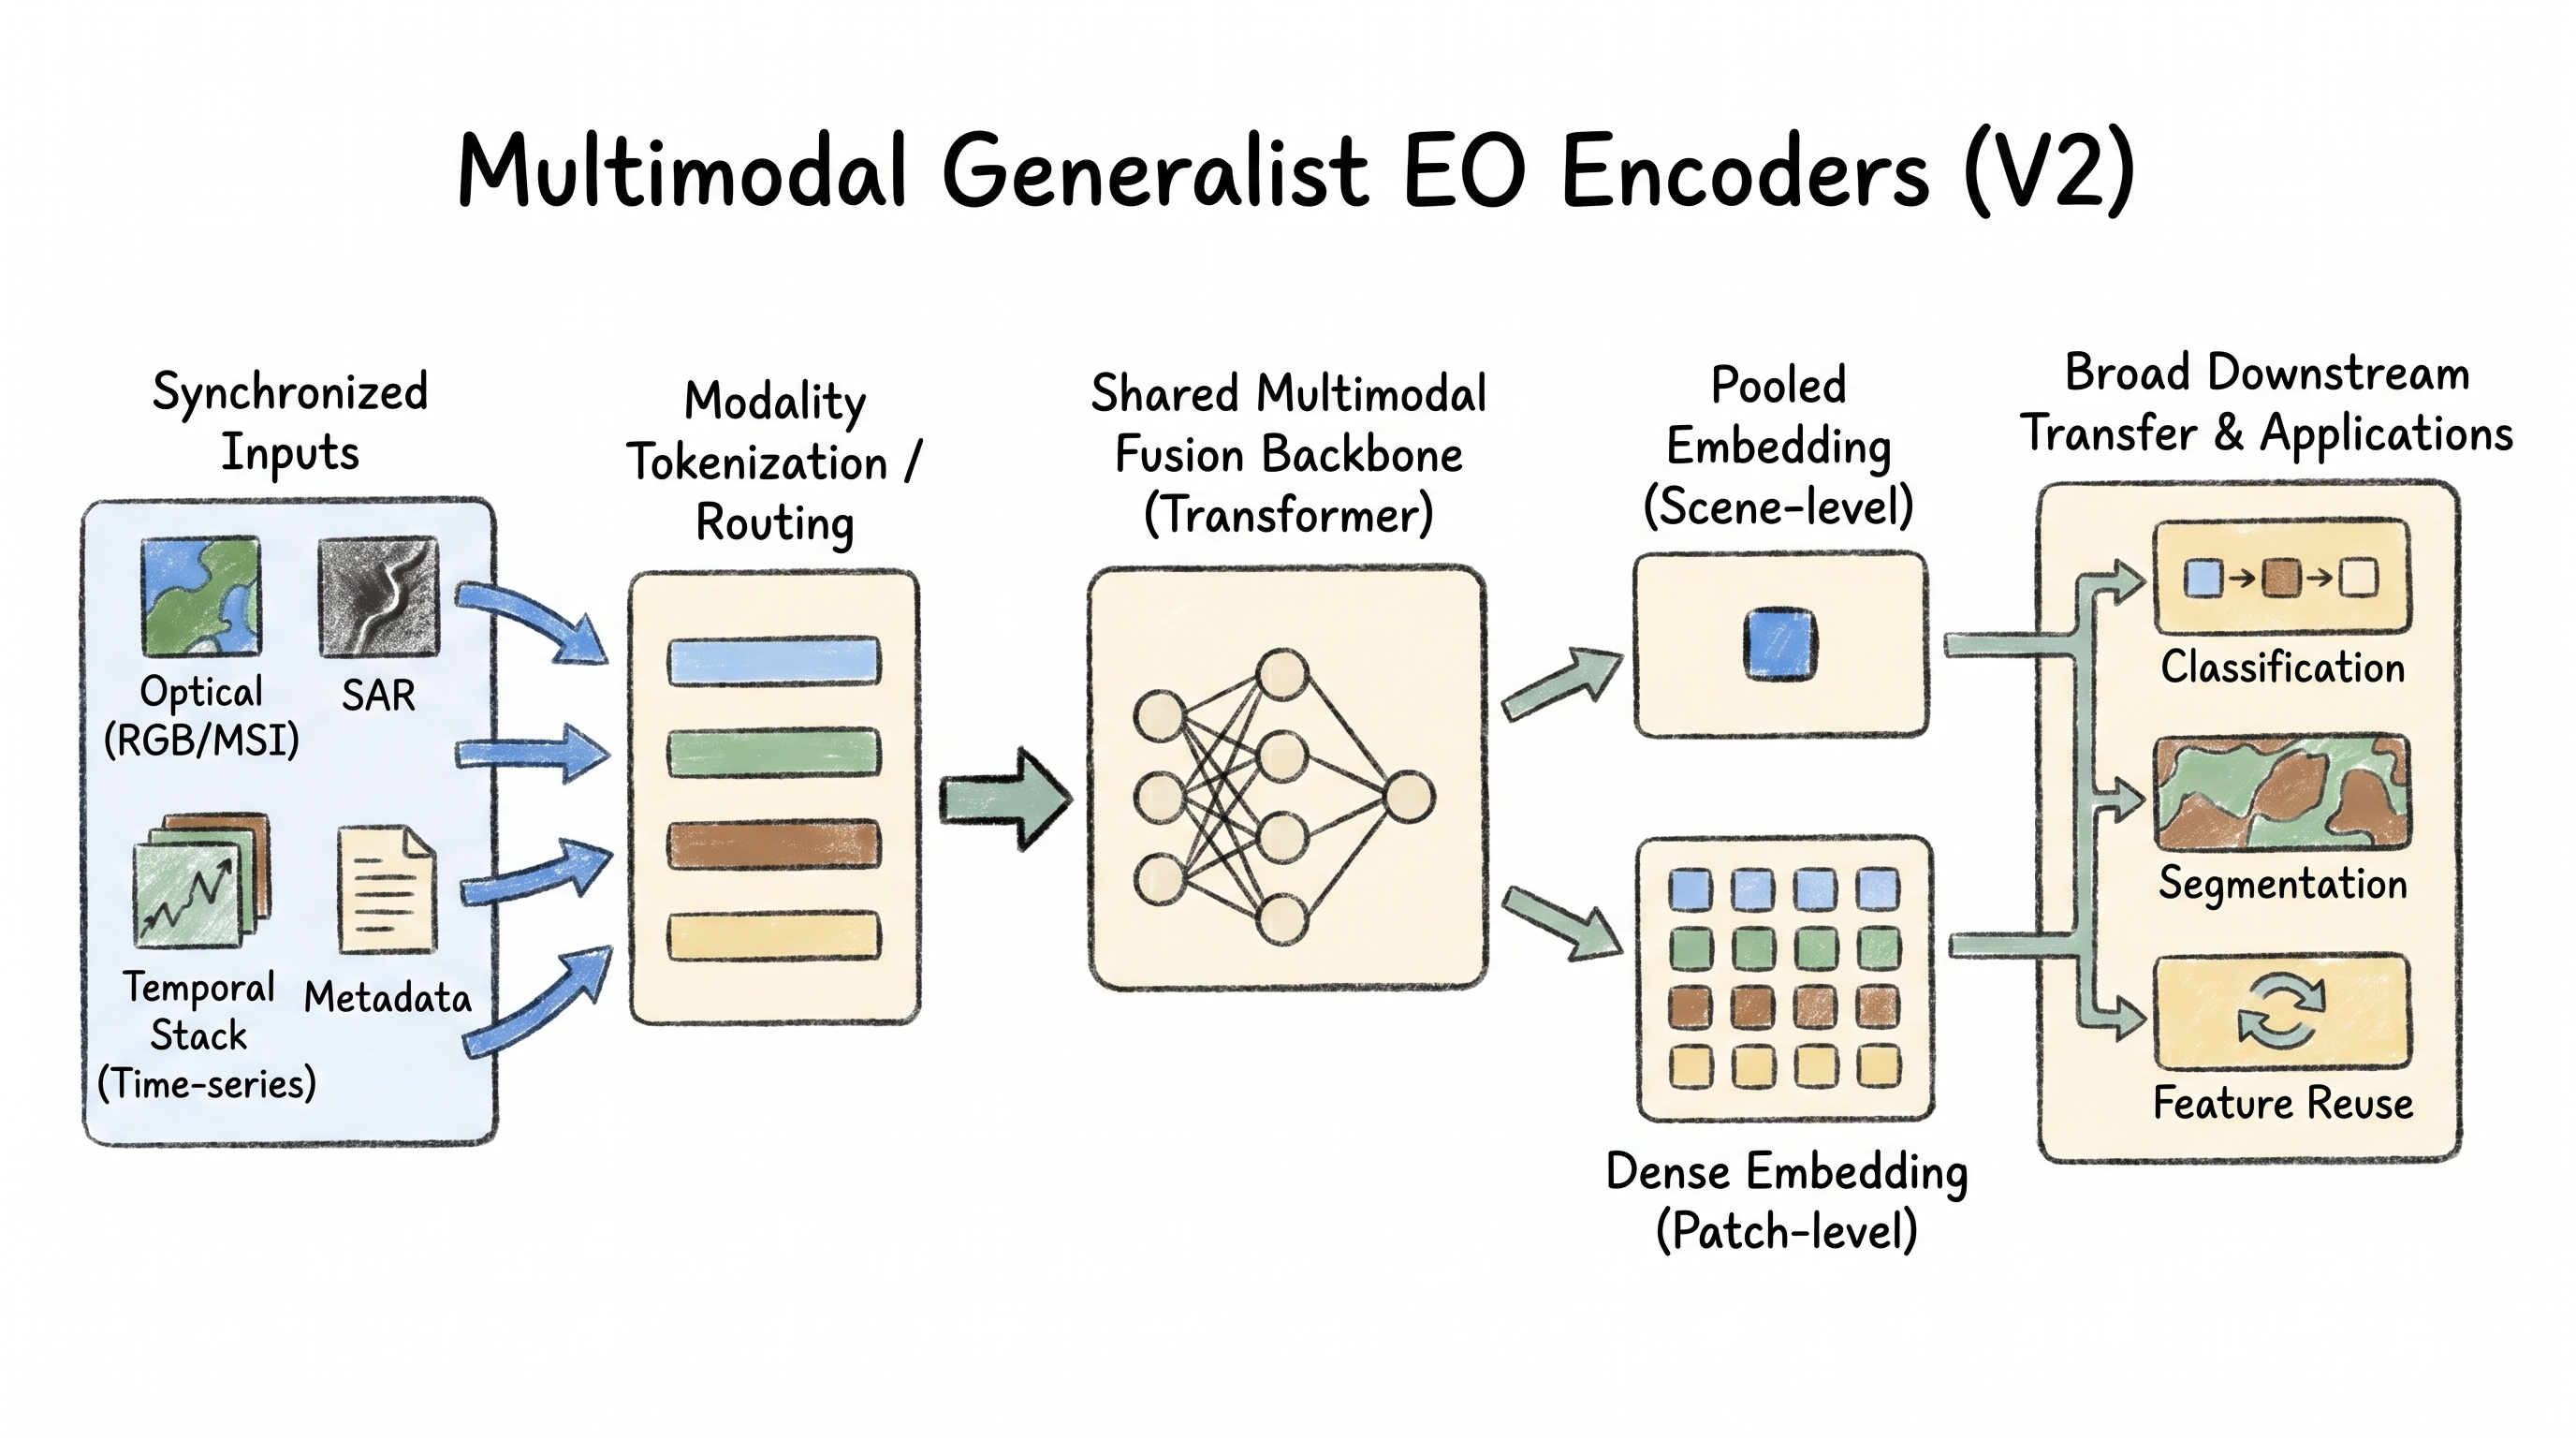
\includegraphics[width=\textwidth]{fig09_family_multimodal_generalist.png}
  \caption{Unified architecture sketch for multimodal generalist EO encoders. Multiple sensor streams are tokenized, routed or aligned, fused by a shared backbone, and exported as pooled or dense representations for broad downstream transfer.}
  \label{fig:family-generalist}
\end{figure}

\paragraph{Architecture summary.}
The defining goal of this family is not simply to process more inputs, but to learn a common representation space across sensors, scales, time, and metadata. Architecturally, that often means modality-specific tokenization combined with a shared transformer or fusion backbone. These models are closest to a true Earth observation foundation layer because they seek one latent space that remains useful under heterogeneous sensing conditions.

\paragraph{Pseudo-code template.}
\begin{pseudocode}
Input:
  modalities {x_1, x_2, ..., x_m}
  temporal or metadata context c

for each modality x_i:
    t_i <- modality_tokenizer_i(x_i, c)

t_shared <- temporal_align_and_route({t_i}, c)
h <- multimodal_backbone(t_shared)
z_pool, z_grid <- readout(h)
optimize self-supervised or multimodal objective

return shared embeddings for cross-sensor downstream transfer
\end{pseudocode}

\subsection{Family V: Domain-specialized embedding models}

Not all useful satellite embeddings aim at maximal generality. AgriFM, FoMo, THOR, and SatVision show that domain-oriented models can remain highly valuable when their sensor assumptions and application context are well matched \citep{agrifm,fomo,thor,satvision}. In a remote sensing review, these models should appear as a major family rather than as outliers, because they often reflect the real structure of EO practice: agriculture, forestry, biodiversity, atmosphere, climate, and societal monitoring all impose different representation demands.

\begin{figure}[t]
  \centering
  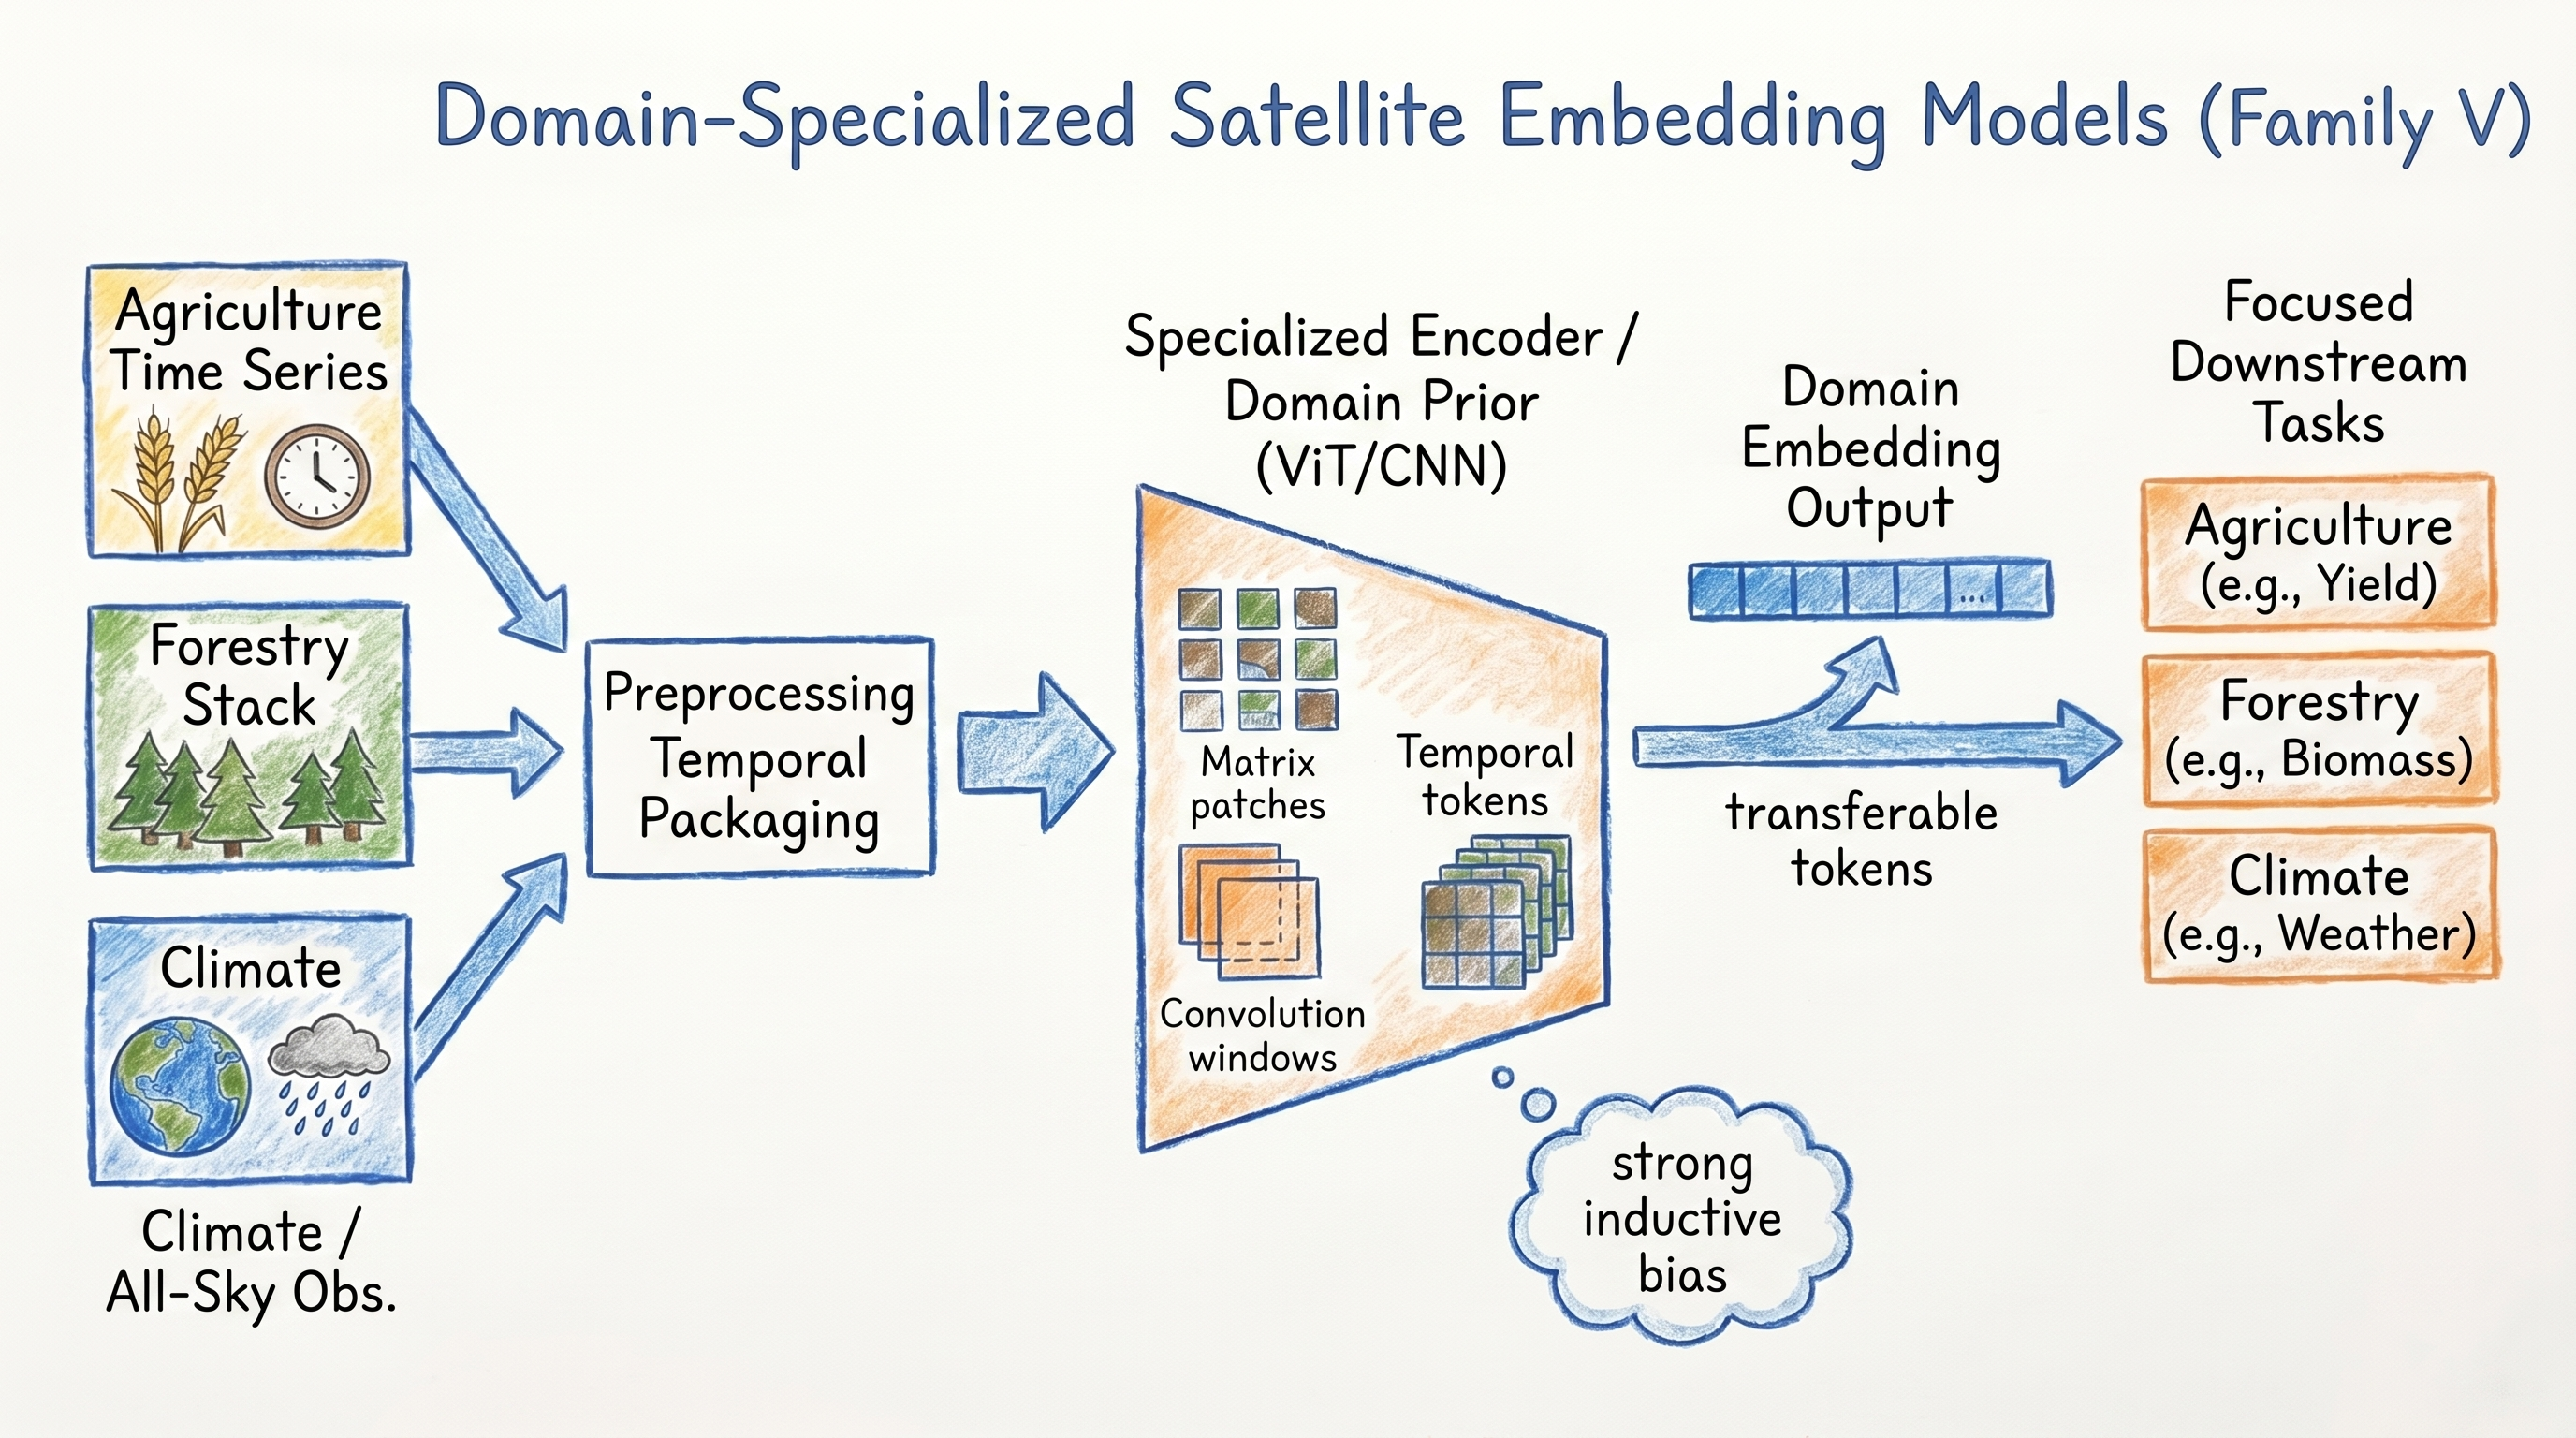
\includegraphics[width=\textwidth]{fig10_family_specialized.png}
  \caption{Unified architecture sketch for domain-specialized satellite embedding models. Domain-specific sensing pipelines and inductive biases are used to produce embeddings that are narrower in scope but often better matched to particular application regimes.}
  \label{fig:family-specialized}
\end{figure}

\paragraph{Architecture summary.}
This family accepts a narrower operating domain in exchange for stronger inductive bias. Agricultural time series, forest monitoring stacks, climate-oriented inputs, or coarse all-sky observations are processed with task-aware temporal packaging, scale handling, or specialized supervision. These models remind us that the best EO embedding is not always the most general one; in many real applications, domain fit matters more than universality.

\paragraph{Pseudo-code template.}
\begin{pseudocode}
Input:
  domain-specific sensor stream x
  domain labels or weak supervision y
  domain prior pi

x_tilde <- domain_preprocess(x, pi)
h <- specialized_encoder(x_tilde, pi)
z <- domain_embedding_head(h)
loss <- domain_objective(z, y, pi)
update model parameters

at deployment:
  reuse z for domain-focused mapping, monitoring, or regression
\end{pseudocode}

\subsection{Cross-family comparison}

After the family-level discussion, the review can return to a unified comparison table. This ordering is closer to the way remote sensing surveys are usually read: first understand the main branches of the field, then inspect the full inventory.

Table~\ref{tab:model-catalog} turns the structured dossier into a paper-ready catalog. Unlike a compact leaderboard, it keeps the deployment type, sensing assumptions, temporal semantics, and pretraining regime visible, because these details strongly determine whether a model is suitable for retrieval, dense prediction, or operational mapping. Appendix Table~\ref{tab:model-appendix-catalog} extends this inventory with authorship, task hints, runtime, GPU memory, and implementation-facing metadata.

\begin{landscape}
\scriptsize
\setlength{\LTleft}{0pt}
\setlength{\LTright}{0pt}
\setlength{\tabcolsep}{3pt}
\renewcommand{\arraystretch}{1.15}
\begin{longtable}{p{1.45cm}p{0.75cm}p{1.2cm}p{0.95cm}p{2.25cm}p{2.05cm}p{2.75cm}p{2.35cm}p{2.25cm}p{1.55cm}p{3.0cm}}
\caption{Comprehensive model summary for the \modelcount{} canonical satellite embedding models currently exposed in \texttt{rs-embed}. The table emphasizes deployment-relevant details rather than only benchmark scores.}\label{tab:model-catalog}\\
\toprule
Model & Year & Venue & Type & Family & Backbone & Sensors / data & Resolution & Temporal semantics & Emb. / output & Pretraining signal \\
\midrule
\endfirsthead
\caption[]{Comprehensive model summary for the canonical \texttt{rs-embed} model set (continued).}\\
\toprule
Model & Year & Venue & Type & Family & Backbone & Sensors / data & Resolution & Temporal semantics & Emb. / output & Pretraining signal \\
\midrule
\endhead
\bottomrule
\endfoot
tessera & 2026 & CVPR & precomputed & Precomputed temporal embedding field & field model over surface spectra embeddings & surface spectra product & 10 m precomputed embedding tiles & annual lookup over product years & 128; pooled, grid & embedding field regression / product training \\
gse & 2025 & arXiv & precomputed & Precomputed annual embedding product & embedding field model & Google Satellite Embedding annual product & 10 m annual embedding product & strict yearly product & 64; pooled, grid & global embedding field learning from sparse labels \\
copernicus & 2025 & ICCV & precomputed & Precomputed foundation map & Copernicus foundation model product & Copernicus product stack & 0.25\textdegree{} precomputed grid & static in current adapter (2021 only) & 768; pooled, grid & foundation model pretraining followed by product distillation \\
remoteclip & 2024 & IEEE TGRS & on-the-fly & Vision-language satellite embedding & CLIP / ViT-B-32 & Sentinel-2 RGB, remote sensing captions, UAV imagery in pretraining & 10 m; Sentinel-2 RGB & single composited observation window at inference & 768; pooled, grid & contrastive image-text alignment (InfoNCE) \\
satmae & 2022 & NeurIPS & on-the-fly & Masked autoencoder for temporal or multispectral EO & ViT-MAE & Sentinel-2 RGB or multispectral/time-series variants in original paper & 10 m; Sentinel-2 RGB & explicit temporal embeddings in the original paper; rs-embed adapter currently uses RGB composite path & 1024; pooled, grid & masked autoencoding with temporal/spectral positional encoding \\
satmaepp & 2024 & CVPR & on-the-fly & Improved masked autoencoder for EO & ViT-L / SatMAE++ & Sentinel-2 RGB in adapter, multispectral Sentinel-2 in paper & 10 m; Sentinel-2 RGB & single composited observation window in adapter & 1024; pooled, grid & revised MAE pretraining for multispectral satellite imagery \\
satmaepp\_s2\_10b & 2024 & CVPR & on-the-fly & Grouped-channel multispectral masked autoencoder & ViT-L / grouped-channel SatMAE++ & Sentinel-2 SR 10-band & 10 m; Sentinel-2 SR 10-band input & single composited observation window in adapter & 1024; pooled, grid & grouped-channel masked autoencoding \\
scalemae & 2023 & ICCV & on-the-fly & Scale-aware masked autoencoder & ViT-L / MAE & Sentinel-2 RGB in adapter, multiscale EO imagery in paper & 10 m; Sentinel-2 RGB, plus explicit semantic scale input & single composited observation window & 1024; pooled, grid & masked autoencoding with explicit resolution conditioning \\
anysat & 2025 & CVPR & on-the-fly & Generalist multi-resolution multimodal EO encoder & versatile JEPA-style EO encoder & Sentinel-2, Sentinel-1, aerial/VHR and other modalities in original paper & 10 m Sentinel-2 time-series input; default per-frame resize 24 px & multi-frame optical sequence with date tokens & 768; pooled, grid & self-supervised representation learning across many configurations \\
galileo & 2025 & ICML & on-the-fly & Global-local multimodal time-series encoder & transformer with global/local branches & Sentinel-2 time series, multiple remote sensing modalities in original work & 10 m Sentinel-2 time-series input; default frame size 64 px, patch size 8 & explicit month tokens and frame masks & 128; pooled, grid & self-supervised multimodal representation learning \\
wildsat & 2025 & ICCV & on-the-fly & Remote sensing representation learning from weak labels & ViT-B-16 & Sentinel-2 RGB, wildlife observations as supervision & 10 m; Sentinel-2 RGB & single composited optical patch & 256; pooled, grid & supervised / weakly supervised representation learning from wildlife observations \\
prithvi & 2023 & arXiv & on-the-fly & Generalist geospatial foundation model & ViT / masked autoencoder lineage & HLS / Sentinel-Landsat style 6-band optical imagery & 30 m in current adapter; Sentinel-2 6-band input & explicit temporal coordinates in adapter and paper family & 768; pooled, grid & self-supervised geospatial pretraining \\
terrafm & 2026 & ICLR & on-the-fly & Unified multisensor foundation model & multisensor transformer & Sentinel-2, Sentinel-1 & 10 m for both S2 and S1 paths; image resized to 224 px & single observation window in current adapter; paper focuses on multisensor unification & 768; pooled, grid & scalable unified multisensor pretraining \\
terramind & 2025 & ICCV & on-the-fly & Generative multimodal EO foundation model & large-scale generative multimodal transformer & Sentinel-2 in adapter, wider multimodal EO stack in paper & 10 m; Sentinel-2 SR 12-band input; image resized to 224 px & single composited optical path in adapter & 384; pooled, grid & large-scale generative multimodal learning \\
dofa & 2024 & arXiv & on-the-fly & Wavelength-aware multimodal foundation model & transformer with neural plasticity / dynamic wavelength handling & multispectral and hyperspectral style inputs, Sentinel-2 in adapter & 10 m for S2 path; fixed resize to 224 px & single observation window in adapter & 768; pooled, grid & self-supervised multimodal EO foundation modeling \\
fomo & 2025 & AAAI & on-the-fly & Forest-oriented multimodal and multiscale foundation model & multimodal transformer / representation learner & Sentinel-2 SR in adapter, multiple scales and tasks in original work & 10 m; Sentinel-2 SR 12-band input; default image size 64 px & single optical composite in adapter & 768; pooled, grid & multi-task forest monitoring pretraining \\
thor & 2026 & arXiv & on-the-fly & Versatile EO foundation model for climate and society & versatile transformer & Sentinel-2 SR 10-band & 10 m; Sentinel-2 SR 10-band input; default image size 288 px & single optical composite in adapter & 768; pooled, grid & foundation pretraining for climate and society applications \\
agrifm & 2026 & Remote Sensing of Environment & on-the-fly & Agriculture-specific multi-source temporal foundation model & Video Swin Transformer & Sentinel-2 in adapter, Sentinel-2, Landsat-8/9, MODIS in original paper & 10 m Sentinel-2 time-series input; default image size 224 px with fixed T-frame packaging & fixed-length multi-frame temporal stack & 1024; pooled, grid & supervised land-cover fraction pretraining with EMA teacher \\
satvision & 2024 & arXiv & on-the-fly & Coarse-resolution all-sky foundation model & SwinV2-style encoder & MODIS 14-band TOA & 1000 m; 14-channel TOA input & single coarse-resolution observation window in adapter & 4096; pooled, grid & foundation pretraining on all-sky MODIS TOA data \\
\end{longtable}
\normalsize
\end{landscape}


Three contrasts recur across families. First, precomputed layers prioritize access and coverage, while on-the-fly encoders prioritize flexibility. Second, multimodal and time-aware systems attempt to absorb sensor heterogeneity at training time, whereas narrower families often compensate with stronger specialization and simpler deployment. Third, vision-language models add open-vocabulary semantics that are mostly absent from pure masked reconstruction pipelines. These contrasts matter more for a review paper than a single benchmark leaderboard, because they explain why different families remain competitive under different downstream conditions.

\begin{figure}[t]
  \centering
  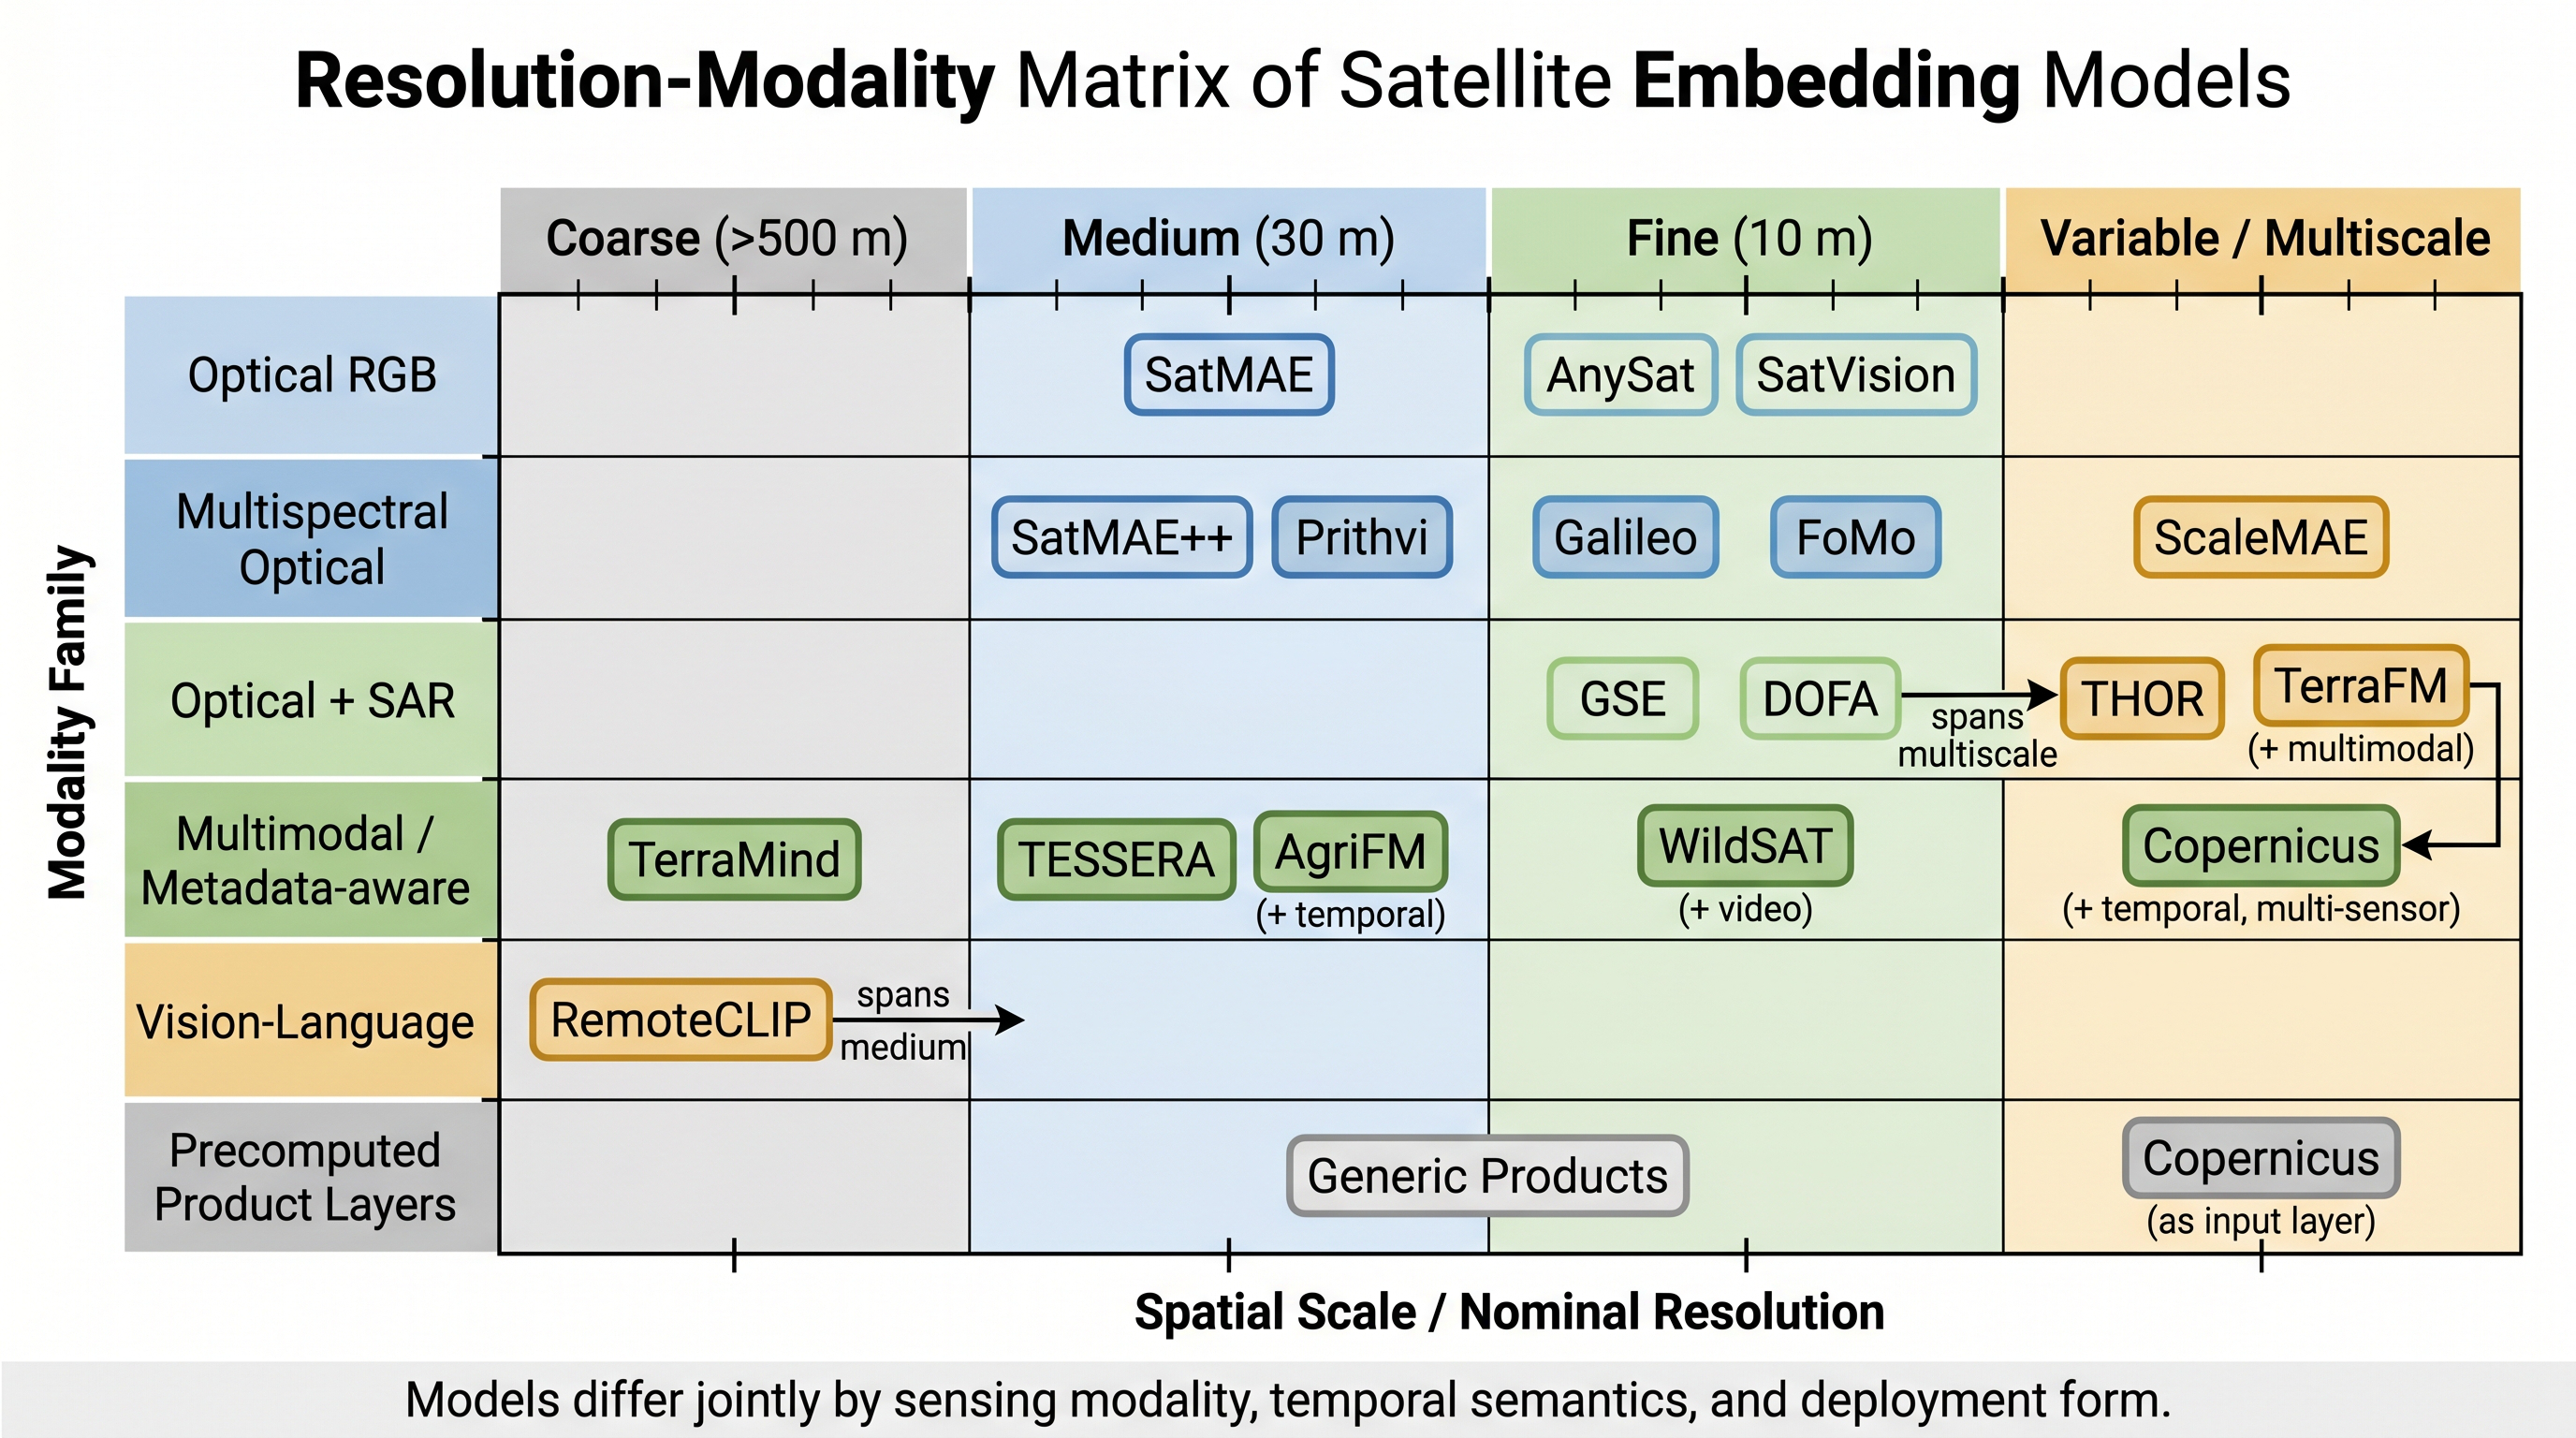
\includegraphics[width=\textwidth]{fig05_resolution_modality_matrix.png}
  \caption{Resolution-modality matrix for current satellite embedding models. The same model family can occupy very different parts of the sensing space, from coarse-resolution all-sky imagery to high-resolution optical-SAR or multimodal temporal embeddings.}
  \label{fig:resolution-modality-matrix}
\end{figure}

Figure~\ref{fig:resolution-modality-matrix} closes this section by summarizing the sensing space covered by current models. In a remote sensing context, this figure is often more informative than a single ranking table because it makes sensor assumptions and scale mismatch immediately visible.

\section{Data Resources and Application Space}

Existing satellite embeddings are already used across a wide range of downstream settings, but the literature often mixes tasks with very different supervision, output granularity, and deployment constraints. A remote sensing review usually benefits from connecting application space back to the data resources and sensor regimes that produced the embeddings in the first place.

\subsection{Pretraining data and sensor regimes}

Current models are built on a few recurring data regimes: medium-resolution optical archives such as Sentinel-2 and Landsat; optical-SAR combinations centered on Sentinel-1 and Sentinel-2; multimodal stacks that combine imagery with metadata, elevation, weather, or labels; and precomputed annual product layers. The choice of data regime strongly shapes what type of embedding can be learned, which downstream tasks transfer well, and how much temporal or cross-sensor flexibility remains at deployment time.

\subsection{Classification and mapping}

The most common use is still transfer to classification-style mapping tasks, including land cover, crop type, forest condition, and other regional labels. Here pooled embeddings are often sufficient, and simple linear probes already reveal large differences in representation quality. This is the mandatory baseline in the proposed benchmark because it is shared across all model families.

\subsection{Segmentation and dense prediction}

Dense token grids or spatially structured product layers support water extraction, land-cover segmentation, flood extent mapping, and similar pixel-level tasks. Not all models expose dense outputs in the same form, which makes segmentation a useful but secondary benchmark axis. It reveals whether spatial structure is preserved in the representation rather than collapsed too early by pooling.

\subsection{Regression and continuous estimation}

Many practical Earth observation tasks are continuous rather than categorical: canopy height, biomass, built-up fraction, crop yield proxies, or environmental indices. Regression therefore provides a cleaner view of whether an embedding preserves smoothly varying physical or semantic structure. It is also compatible with both precomputed annual layers and on-the-fly encoders.

\subsection{Retrieval and multimodal interaction}

Vision-language or broader multimodal representations enable text-to-region retrieval, cross-modal search, and weakly supervised triage. These use cases are particularly relevant for systems such as RemoteCLIP and WildSAT, but they also motivate future extensions for metadata-aware or instruction-conditioned EO representation learning.

\subsection{Operational considerations}

Application fit depends on more than headline accuracy. Practitioners must also account for native spatial scale, time coverage, whether embeddings are analysis-ready products, and whether dense outputs can be produced under realistic memory budgets. This is one reason the benchmark in this repository records runtime and peak memory alongside downstream metrics.

\section{Comparative Evaluation Protocol}

To move beyond narrative comparison, the review includes a compact benchmark design centered on a single mixed study area. The current pilot region is the Wuhan East Lake and Tangxun Lake corridor in China, selected because it combines urban fabric, water bodies, cropland, and vegetation within a limited spatial extent. This diversity makes it possible to study several downstream tasks without switching datasets or geographic context.

\subsection{Pilot study area}

The Wuhan pilot is not intended to replace global benchmarks. Its role is to provide one controlled, mixed-landscape setting in which multiple embedding families can be compared under shared spatial context, labels, and extraction windows.

\subsection{Benchmark tasks and protocol}

The first benchmark pass uses three task families:

\begin{enumerate}[leftmargin=1.4em]
  \item tile classification over coarse WorldCover classes;
  \item water segmentation with JRC Global Surface Water or Dynamic World labels;
  \item tile-level fraction regression for built-up or vegetation proportion.
\end{enumerate}

All models use the same tile centroids, train/validation/test split, and lightweight probe heads. Annual product models are evaluated at the nearest available year, while on-the-fly models use a common Sentinel-2 temporal window. Encoder weights remain frozen in the first pass so that the benchmark measures representation quality rather than fine-tuning capacity.

\begin{figure}[t]
  \centering
  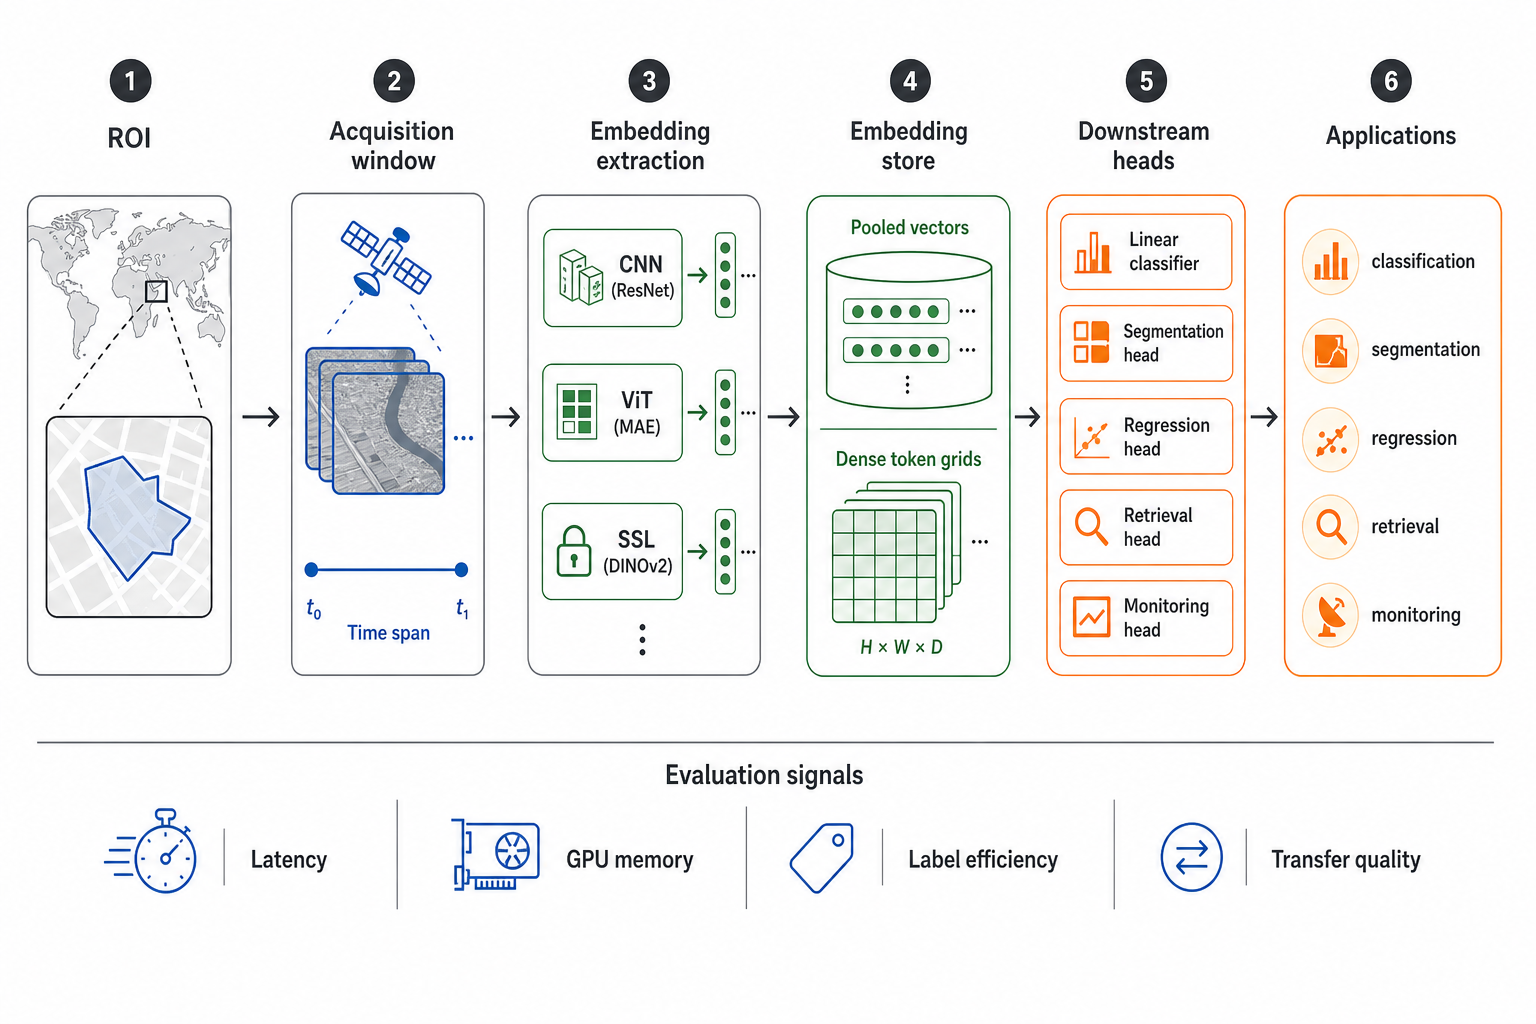
\includegraphics[width=\textwidth]{fig02_application_pipeline_gptimage2_20260502.png}
  \caption{Application-oriented benchmark pipeline. A shared region of interest is converted into a unified embedding extraction workflow, lightweight probe heads, and downstream evaluation targets spanning classification, segmentation, regression, and retrieval.}
  \label{fig:application-pipeline}
\end{figure}

\subsection{Why a small-area protocol is still informative}

A compact benchmark cannot replace global evaluation, but it can reveal the practical trade-offs that matter most during model selection. Specifically, it highlights scale mismatch, the effect of temporal summarization, and the difference between pooled-only and dense-capable representations. It also lowers the cost of iteration, making it easier to add new models or new downstream heads as the repository evolves. Figure~\ref{fig:application-pipeline} shows the intended experiment flow that will populate the comparison tables in the next draft.

\subsection{Expected outputs}

The benchmark should produce one table that combines quality and runtime, a quality-versus-latency figure, and a family-level transfer summary. These artifacts will directly support the application section of the survey and can also feed the interactive explorer described in Section~\ref{sec:system-layer}.

\subsection{First executed pilot}

The first executed pass now uses the Wuhan East Lake ROI already defined in this survey workspace, but with a deliberately conservative task setup chosen to ensure balanced labels and fast iteration. Instead of forcing a sparse 6-class classification problem in a compact urban-water corridor, the executed pilot collapses the label space into three dominant classes: \emph{water}, \emph{green}, and \emph{built}. A regular \(10 \times 10\) candidate grid with 500\,m square buffers was generated inside the ROI, ESA WorldCover 2021 and JRC Global Surface Water were queried through Google Earth Engine, and 15 tiles were selected with a dominance threshold of 0.5, yielding a perfectly balanced subset of 5 tiles per class. The same tiles were then used for tile-level built fraction, green fraction, and water fraction regression.

The first model panel covers one precomputed product model (GSE), one vision-language model (RemoteCLIP), one masked autoencoder model (SatMAE++ S2-10B), one multimodal generalist encoder (Galileo), one domain-specialized temporal model (AgriFM), and one coarse-resolution precomputed product (Copernicus). Table~\ref{tab:wuhan-pilot-results} summarizes the initial results. Two observations are already useful for the review. First, several families can separate the 3-class pilot almost perfectly under frozen linear probing, suggesting that even a small-area benchmark can expose strong transfer behavior quickly. Second, deployment constraints matter as much as accuracy: Copernicus failed not because of a broken implementation, but because its 0.25\(^\circ\) native embedding pixel is fundamentally mismatched to a 500\,m local ROI. This is exactly the kind of scale-and-deployment issue that an embedding-centered review should make visible.

\begin{table*}[t]
\centering
\caption{First executed Wuhan pilot benchmark on a balanced 15-tile subset (5 water, 5 green, 5 built). The pilot uses 500\,m square buffers, frozen pooled embeddings, 3-class dominant land-cover classification, and tile-level fraction regression.}
\label{tab:wuhan-pilot-results}
\small
\begin{tabular}{lcccccc}
\toprule
Model & Status & Macro F1 & Built RMSE & Water RMSE & Time (s) & Peak GPU MB \\
\midrule
GSE & pass & 1.000 & 0.061 & 0.348 & 35.6 & 0.0 \\
SatMAE++ S2-10B & pass & 1.000 & 0.083 & 0.264 & 36.9 & 1353.8 \\
Galileo & pass & 1.000 & 0.161 & 0.305 & 87.6 & 277.3 \\
AgriFM & pass & 1.000 & 0.238 & 0.836 & 88.7 & 591.1 \\
RemoteCLIP & pass & 0.852 & 0.187 & 0.300 & 44.6 & 602.6 \\
Copernicus & fail & --- & --- & --- & --- & --- \\
\bottomrule
\end{tabular}
\end{table*}


\section{System Layer and Interactive Access}
\label{sec:system-layer}

An embedding survey is substantially more useful when readers can move from the paper to a runnable interface. For that reason, this repository includes a lightweight Leaflet-based prototype that consumes the structured dossier and presents four elements in a single view: a model selector, a pilot region of interest, runtime metadata, and task-oriented interpretation notes.

The intended system architecture has three layers. The first layer stores model metadata, processed paper notes, and benchmark outputs. The second layer exposes embedding extraction, product sampling, and export services behind a uniform API. The third layer provides the browser interface for region selection, model comparison, and rapid task setup. This structure mirrors the logic of the review itself: concepts and model metadata first, benchmarking second, and access tooling third.

\begin{figure}[t]
  \centering
  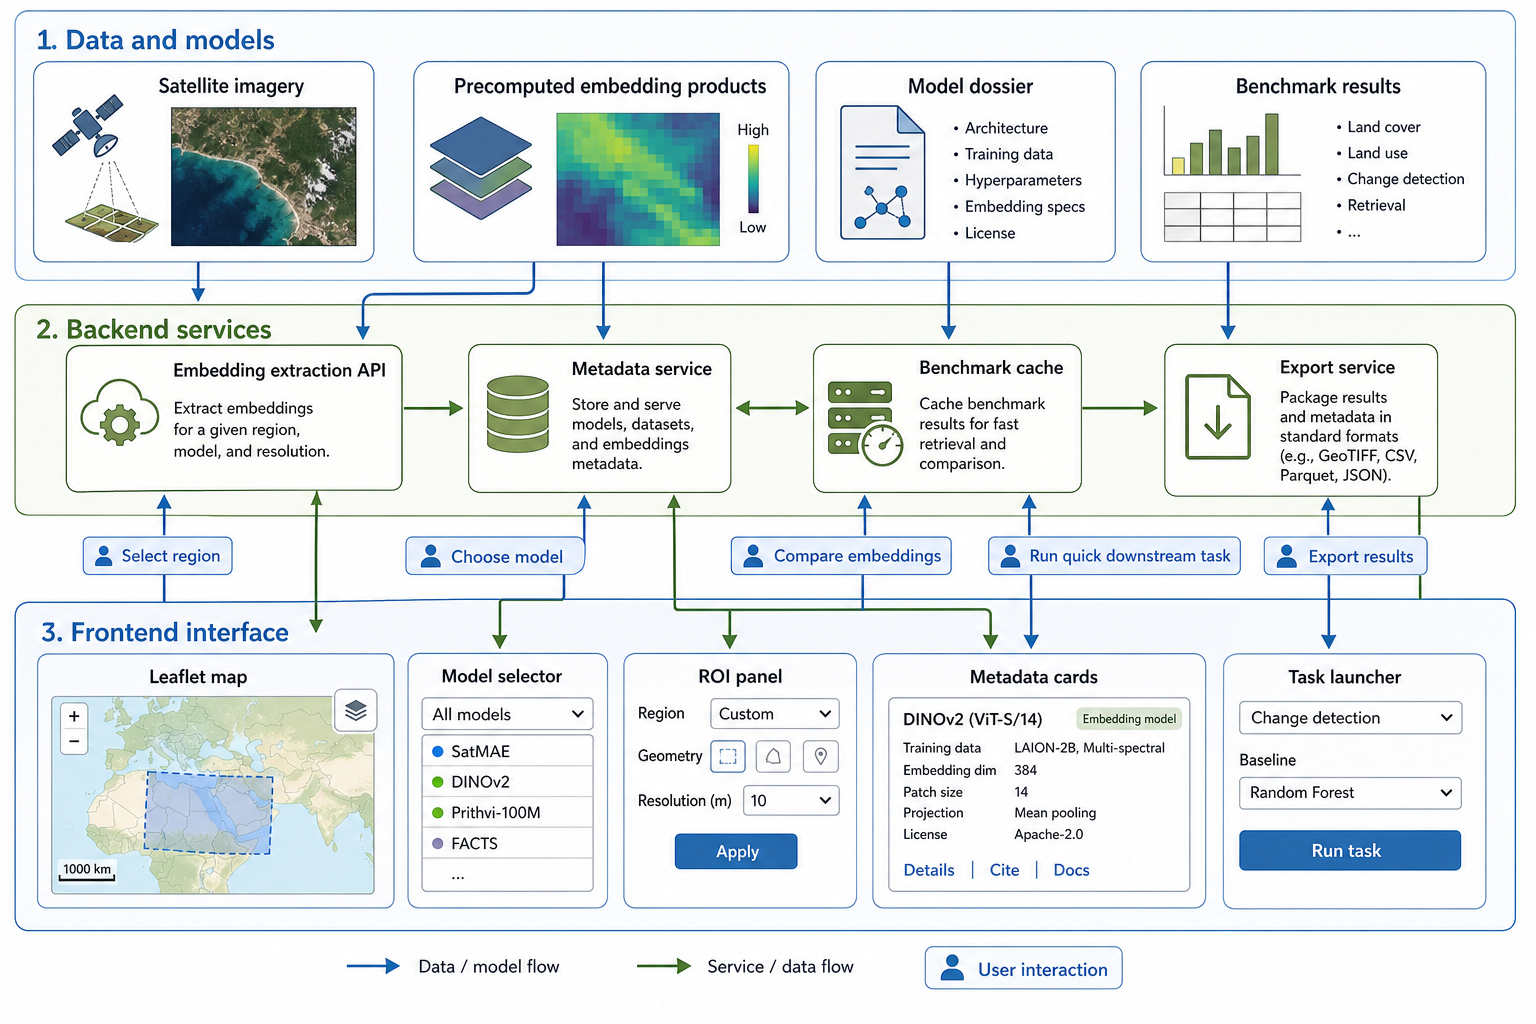
\includegraphics[width=\textwidth]{fig03_system_overview_gptimage2_20260502.png}
  \caption{System layer for the proposed Satellite Embedding Explorer. The same structured assets used by the review can also drive metadata browsing, ROI selection, model comparison, and later benchmark services.}
  \label{fig:system-overview}
\end{figure}

Even the current static prototype is useful because it forces the review assets into machine-readable form. The same \texttt{model\_dossier.json} file can drive paper tables, browser filters, and later benchmarking scripts. This reduces duplication and makes it easier to keep the literature summary synchronized with the software layer.

\section{Challenges and Future Directions}

Several unresolved issues cut across the current satellite embedding landscape.

\paragraph{Temporal ambiguity.}
Many models mix annual products, temporal stacks, and short compositing windows under the same broad label of ``embedding.'' A stronger standard is needed for reporting what time information the representation actually preserves.

\paragraph{Scale mismatch.}
Embeddings generated at 10\,m, 30\,m, 1\,km, or 0.25$^\circ$ are not interchangeable, even when they are benchmarked on nominally similar tasks. A review must therefore report native scale explicitly and treat resampling as a methodological choice rather than a neutral preprocessing step.

\paragraph{Product versus model comparison.}
Precomputed layers and on-the-fly encoders are often compared as if they were the same object. They are not. Products optimize access and reuse, whereas checkpoints optimize flexibility. Future work should evaluate these regimes with metrics that acknowledge both predictive quality and deployment cost.

\paragraph{Application realism.}
Most current benchmarking practice still favors standard datasets over operational mapping settings. Embedding evaluation would benefit from more geographically grounded protocols, richer regression tasks, and stronger attention to low-label and cross-year transfer.

\paragraph{Open interfaces.}
The field lacks a common access layer analogous to model hubs in natural image or language processing. A robust embedding interface should expose not only the checkpoint but also sensor assumptions, temporal requirements, output forms, and recommended downstream usage patterns.

\section{Conclusion}

Satellite embeddings are emerging as a practical abstraction layer for Earth observation, but the surrounding literature is still fragmented across architecture families, sensor regimes, and product formats. This review addresses that gap by organizing the area around the representation itself rather than around any single training paradigm. The resulting framework combines a taxonomy, a model dossier, a benchmark plan, and an interactive access layer.

The immediate next step is empirical: execute the small-area benchmark and convert the outputs into the comparison tables and figures planned in this draft. Once those results are in place, the survey can move from a structured framework to a complete evidence-backed review that is useful both to readers of the literature and to practitioners choosing an embedding for real geospatial workflows.

\appendix
\section{Extended Model Inventory}

Table~\ref{tab:model-appendix-catalog} expands the main-text catalog with implementation-oriented details that are useful during reproduction, model selection, and future benchmark scripting. In particular, it keeps author lists, output modes, typical tasks, runtime, GPU memory, and code or artifact availability visible in one place.

\begin{landscape}
\scriptsize
\setlength{\LTleft}{0pt}
\setlength{\LTright}{0pt}
\setlength{\tabcolsep}{3pt}
\renewcommand{\arraystretch}{1.12}
\begin{longtable}{p{1.35cm}p{2.9cm}p{2.25cm}p{1.95cm}p{1.65cm}p{2.3cm}p{1.45cm}p{1.35cm}p{2.7cm}p{1.95cm}}
\caption{Extended implementation-oriented inventory for the canonical \texttt{rs-embed} model set. This appendix table adds authorship, output modes, application hints, and runtime metadata beyond the main-text catalog.}\label{tab:model-appendix-catalog}\\
\toprule
Model & Authors & Inputs / modalities & Time coverage & Outputs & Typical tasks & Elapsed (s) & Peak GPU (MB) & Code / artifact & Training data summary \\
\midrule
\endfirsthead
\caption[]{Extended implementation-oriented inventory for the canonical \texttt{rs-embed} model set (continued).}\\
\toprule
Model & Authors & Inputs / modalities & Time coverage & Outputs & Typical tasks & Elapsed (s) & Peak GPU (MB) & Code / artifact & Training data summary \\
\midrule
\endhead
\bottomrule
\endfoot
tessera & Zhengpeng Feng, Clement Atzberger, Sadiq Jaffer, Jovana Knezevic, Silja Sormunen, Robin Young, Madeline C. Lisaius, Markus Immitzer, James Ball, David A. Coomes, Anil Madhavapeddy, Andrew Blake, Srinivasan Keshav & surface spectra product & 2017-2025 & pooled, grid & representation lookup, regional embedding analysis, retrieval, downstream transfer & 1025.79 & 0.0 & GitHub & global Earth observation spectra aggregated into tessellated embedding tiles \\
gse & Christopher F. Brown, Michal R. Kazmierski, Valerie J. Pasquarella, William J. Rucklidge, Masha Samsikova, Chenhui Zhang, Evan Shelhamer, Estefania Lahera, Olivia Wiles, Simon Ilyushchenko, Noel Gorelick, Lihui Lydia Zhang, Sophia Alj, Emily Schechter, Sean Askay, Oliver Guinan, Rebecca Moore, Alexis Boukouvalas, Pushmeet Kohli & Google Satellite Embedding annual product & 2017-2024 & pooled, grid & global mapping, rapid transfer, feature sampling & 4.46 & 0.0 & Earth Engine catalog & global annual satellite embedding product served through Earth Engine \\
copernicus & Yi Wang, Zhitong Xiong, Chenying Liu, Adam J. Stewart, Thomas Dujardin, Nikolaos Ioannis Bountos, Angelos Zavras, Franziska Gerken, Ioannis Papoutsis, Laura Leal-Taixe, Xiao Xiang Zhu & Copernicus product stack & 2021 only & pooled, grid & broad-area retrieval, feature extraction, downstream transfer & 11.52 & 0.0 & Hugging Face & global Copernicus-scale EO data compiled into a unified feature raster \\
remoteclip & Fan Liu, Delong Chen, Zhangqingyun Guan, Xiaocong Zhou, Jiale Zhu, Qiaolin Ye, Liyong Fu, Jun Zhou & Sentinel-2 RGB, remote sensing captions, UAV imagery in pretraining & S2\_SR\_HARMONIZED & pooled, grid & zero-shot classification, retrieval, few-shot classification, counting, open-vocabulary transfer & 13.87 & 600.8 & GitHub & large image-caption corpus built via box-to-caption and mask-to-caption conversion plus UAV imagery \\
satmae & Yezhen Cong, Samar Khanna, Chenlin Meng, Patrick Liu, Erik Rozi, Yutong He, Marshall Burke, David B. Lobell, Stefano Ermon & Sentinel-2 RGB or multispectral/time-series variants in original paper & S2\_SR\_HARMONIZED & pooled, grid & classification, segmentation, transfer learning, representation learning & 2061.66 & 1276.6 & GitHub & fMoW-Sentinel and satellite imagery with temporal and spectral structure \\
satmaepp & Mubashir Noman, Muzammal Naseer, Hisham Cholakkal, Rao Muhammad Anwer, Salman Khan, Fahad Shahbaz Khan & Sentinel-2 RGB in adapter, multispectral Sentinel-2 in paper & S2\_SR\_HARMONIZED & pooled, grid & classification, segmentation, representation transfer & 2052.08 & 1276.7 & GitHub & fMoW RGB / multispectral and remote sensing pretraining corpora \\
satmaepp\_s2\_10b & Mubashir Noman, Muzammal Naseer, Hisham Cholakkal, Rao Muhammad Anwer, Salman Khan, Fahad Shahbaz Khan & Sentinel-2 SR 10-band & S2\_SR\_HARMONIZED & pooled, grid & classification, transfer learning, representation extraction & 17.52 & 1288.5 & GitHub & Sentinel/fMoW-style multispectral pretraining checkpoint \\
scalemae & Colorado J. Reed, Ritwik Gupta, Shufan Li, Sarah Brockman, Christopher Funk, Brian Clipp, Kurt Keutzer, Salvatore Candido, Matt Uyttendaele, Trevor Darrell & Sentinel-2 RGB in adapter, multiscale EO imagery in paper & S2\_SR\_HARMONIZED & pooled, grid & cross-resolution transfer, classification, segmentation & 1874.83 & 1175.0 & GitHub & multiscale geospatial imagery with explicit resolution metadata \\
anysat & Guillaume Astruc, Nicolas Gonthier, Clement Mallet, Loic Landrieu & Sentinel-2, Sentinel-1, aerial/VHR and other modalities in original paper & S2\_SR\_HARMONIZED, split into T frames & pooled, grid & classification, segmentation, cross-modal transfer, few-shot transfer & 789.78 & 550.3 & GitHub & GeoPlex-like multi-resolution multi-modality corpora \\
galileo & Gabriel Tseng, Anthony Fuller, Marlena Reil, Henry Herzog, Patrick Beukema, Favyen Bastani, James R. Green, Evan Shelhamer, Hannah Kerner, David Rolnick & Sentinel-2 time series, multiple remote sensing modalities in original work & S2\_SR\_HARMONIZED, split into T frames & pooled, grid & classification, segmentation, retrieval, time-series transfer & 24.12 & 281.3 & GitHub & many remote sensing modalities with temporal alignment \\
wildsat & Rangel Daroya, Elijah Cole, Oisin Mac Aodha, Grant Van Horn, Subhransu Maji & Sentinel-2 RGB, wildlife observations as supervision & S2\_SR\_HARMONIZED & pooled, grid & ecology transfer, classification, retrieval, representation learning & 666.26 & 348.0 & GitHub & satellite imagery aligned with wildlife observations and biodiversity labels \\
prithvi & Johannes Jakubik, Sujit Roy, C. E. Phillips, Paolo Fraccaro, Denys Godwin, Bianca Zadrozny, Daniela Szwarcman, Carlos Gomes, Gabby Nyirjesy, Blair Edwards, Daiki Kimura, Naomi Simumba, Linsong Chu, S. Karthik Mukkavilli, Devyani Lambhate, Kamal Das, Ranjini Bangalore, Dario Oliveira, Michal Muszynski, Kumar Ankur, Muthukumaran Ramasubramanian, Iksha Gurung, Sam Khallaghi, Hanxi Li, Michael Cecil, Maryam Ahmadi, Fatemeh Kordi, Hamed Alemohammad, Manil Maskey, Raghu Ganti, Kommy Weldemariam, Rahul Ramachandran & HLS / Sentinel-Landsat style 6-band optical imagery & S2\_SR\_HARMONIZED; year is normalized to a full-year range & pooled, grid & classification, segmentation, mapping, generalist transfer & 719.82 & 455.1 & Hugging Face & NASA/IBM geospatial corpora designed for generalist GeoAI \\
terrafm & Muhammad Sohail Danish, Muhammad Akhtar Munir, Syed Roshaan Ali Shah, Muhammad Haris Khan, Rao Muhammad Anwer, Jorma Laaksonen, Fahad Shahbaz Khan, Salman Khan & Sentinel-2, Sentinel-1 & range(...) over either Sentinel-2 or Sentinel-1 collections & pooled, grid & classification, segmentation, cross-sensor transfer, representation learning & 671.25 & 477.7 & GitHub & large multisensor Earth observation corpus spanning S1 and S2 \\
terramind & Johannes Jakubik, Felix Yang, Benedikt Blumenstiel, Erik Scheurer, Rocco Sedona, Stefano Maurogiovanni, Jente Bosmans, Nikolaos Dionelis, Valerio Marsocci, Niklas Kopp, Rahul Ramachandran, Paolo Fraccaro, Thomas Brunschwiler, Gabriele Cavallaro, Juan Bernabe-Moreno, Nicolas Longepe & Sentinel-2 in adapter, wider multimodal EO stack in paper & S2\_SR\_HARMONIZED & pooled, grid & representation learning, generation, multimodal transfer & 725.17 & 104.2 & GitHub & large multimodal Earth observation data for generation and representation learning \\
dofa & Zhitong Xiong, Yi Wang, Fahong Zhang, Adam J. Stewart, Joelle Hanna, Damian Borth, Ioannis Papoutsis, Bertrand Le Saux, Gustau Camps-Valls, Xiao Xiang Zhu & multispectral and hyperspectral style inputs, Sentinel-2 in adapter & S2\_SR\_HARMONIZED & pooled, grid & classification, cross-sensor transfer, hyperspectral transfer & 104.99 & 464.6 & GitHub & multimodal EO corpora with wavelength metadata \\
fomo & Nikolaos Ioannis Bountos, Arthur Ouaknine, Ioannis Papoutsis, David Rolnick & Sentinel-2 SR in adapter, multiple scales and tasks in original work & S2\_SR\_HARMONIZED & pooled, grid & forest type mapping, biomass-related transfer, classification, segmentation & 418.65 & 361.3 & GitHub & forest monitoring corpora across multiple modalities and scales \\
thor & Theodor Forgaard, Jarle Reksten, Anders Waldeland, Valerio Marsocci, Nicolas Longepe, Michael Kampffmeyer, Arnt-Borre Salberg & Sentinel-2 SR 10-band & S2\_SR\_HARMONIZED & pooled, grid & classification, regression, mapping, broad transfer & 555.73 & 489.3 & GitHub & large EO corpus oriented toward broad societal and climate tasks \\
agrifm & Wenyuan Li, Shunlin Liang, Keyan Chen, Yongzhe Chen, Han Ma, Jianglei Xu, Yichuan Ma, Yuxiang Zhang, Shikang Guan, Husheng Fang, Zhenwei Shi & Sentinel-2 in adapter, Sentinel-2, Landsat-8/9, MODIS in original paper & S2\_SR\_HARMONIZED, split into T frames & pooled, grid & cropland mapping, field boundary delineation, crop type mapping, agricultural land-use mapping & 21.30 & 590.3 & GitHub & 25M+ globally sampled multi-source temporal patches from MODIS, Landsat, and Sentinel-2 \\
satvision & Caleb S. Spradlin, Jordan A. Caraballo-Vega, Jian Li, Mark L. Carroll, Jie Gong, Paul M. Montesano & MODIS 14-band TOA & default MODIS/061/MOD021KM & pooled, grid & atmospheric science, environmental monitoring, coarse-resolution transfer & 7179.36 & 9938.2 & GitHub & 14-band MODIS TOA imagery capturing visible, NIR, and thermal bands under all-sky conditions \\
\end{longtable}
\normalsize
\end{landscape}



\bibliographystyle{plainnat}
\bibliography{references}

\end{document}
